%%%%%%%%%%%%%%%%%%%%%%%%%%%%%%%%%%%%%%%%%%%%%%%%%%%%%%%%%
% Niniejszy plik przedstawia przykładowy skład 
% pracy dyplomowej na Wydziale Matematyki PWr. 
% 
% Autorzy: 
% Damian Fafuła
% Michał Kijaczko
% Jakub Michalczak
% Maciej Miśta
% Dagmara Nowak
% Tomasz Skalski
% Wojciech Słomian
%
%% Data utworzenia: 8.05.2018
% Numer wersji: 1
%
% Poniższą formatkę można rozpowszechniać i edytować 
% pod warunkiem zachowania numeru wersji, 
% informacji o autorach i dodaniu informacji 
% o wprowadzonych zmianach.
%
%%%%%%%%%%%%%%%%%%%%%%%%%%%%%%%%%%%%%%%%%%%%%%%%%%%%%%%%%
% Domyślną opcją jest: praca magisterska, język polski.
% W przypadku pracy pisanej w języku angielskim dodajemy 
% opcję [english].
% Dla pracy licencjackiej dodajemy opcję [licencjacka].
% Dla pracy inżynierskiej dodajemy opcję [inzynierska].
% Dopuszczalne są podwójne opcje, np. [licencjacka, english].
% Opcje dodajemy w kwadratowym nawiasie przy \documentclass.
%
%
%%%%%%%%%%%%%%%%%%%%%%%%%%%%%%%%%%%%%%%%%%%%%%%%%%%%%%%%%
\documentclass[inzynierska]{pwr_wmat_praca_dyplomowa}
\frenchspacing 
%%%%%%%%%%%%%%%%%%%%%%%%%%%%%%%%%%%%%%%%%%%%%%%%%%%%%%%%%
%              DANE DO PRACY
%
% W przypadku pracy dyplomowej w języku angielskim nie jest konieczne 
% wypełnianie pól: \tytul{}, \kierunek{}, \specjalnosc{}, 
%                  \streszczenie{}, \slowakluczowe{}.
%%%%%%%%%%%%%%%%%%%%%%%%%%%%%%%%%%%%%%%%%%%%%%%%%%%%%%%%%
%
% Imię i nazwisko autora
\autor{Aleksander Jakóbczyk}
%
% Tytuł pracy dyplomowej 
\tytul{Zastosowanie stochastycznej
	optymalizacji do gier
	częściowo obserwowalnych} 
\tytulang{Application of Stochastic Optimization to Partially Observable Games}
%
% Tytuł / stopień / imię i nazwisko opiekuna
\opiekun{dr inż. Andrzej Giniewicz}
%
% Kierunek studiów wybieramy spośród następujących:
% 1) Matematyka
% 2) Matematyka i Statystyka
% 3) Matematyka stosowana
\kierunekstudiow{Matematyka stosowana}
%
% Kierunek studiów po angielsku wybieramy spośród następujących:
% 1) Mathematics
% 2) Mathematics and Statistics
% 3) Applied Mathematics
\kierunekstudiowang{Mathematics}
%
% Specjalność wybieramy spośród następujących: 
% KIERUNEK: Matematyka
% 1) Matematyka teoretyczna,
% 2) Statystyka matematyczna,
% 3) Matematyka finansowa i ubezpieczeniowa,
%
% KIERUNEK: Matematyka i Statystyka
% 4) Matematyka,
% 5) Statystyka i analiza danych, 
%
% 6) -- (w przypadku braku specjalizacji).
\specjalnosc{--} 
%
% Specjalność w języku angielskim wybieramy spośród następujących:
% KIERUNEK: Matematyka
% 1) Theoretical Mathematics,
% 2) Mathematical Statistics,
% 3) Financial and Actuarial Mathematics,
%
% KIERUNEK: Matematyka i Statystyka
% 4) Mathematics,
% 5) Statistics and Data Analysis,
%
% KIERUNEK: Applied Mathematics
% 6) Financial and Actuarial Mathematics, 
% 7) Mathematics for Industry and Commerce,
% 8) Computational Mathematics,
% 9) Modelling, Simulation and Optimization.
%
% 10) -- (w przypadku braku specjalizacji).
\specjalnoscang{Theoretical Mathematics} 
%
% Krótkie streszczenia po polsku i angielsku
% - nie dłuższe niż 530 znaków.

\streszczenie{Celem pracy jest wyznaczenie nieoczekiwanych strategii w grach częściowo obserwowalnych za pomocą metod stochastycznej optymalizacji.
%! wstemp do poprawy
W pracy zostały zaproponowane nowe algorytmy, pozwalające na szybsze wyznaczenie strategii optymalnej. Zaproponowano również kolejny algorytm generacyjny. Przeprowadzona została analiza porównawcza kilku wybranych metod optymalizacji.}
\streszczenieang{The aim of this work is to determine unexpected strategies in partially observable games using stochastic optimization methods. New algorithms have been proposed to allow for faster determination of the optimal strategy. Another generative algorithm has been proposed. A comparative analysis of several optimization methods was conducted.}
%
% Podajemy najważniejsze słowa kluczowe po polsku i angielsku
% - w obu przypadkach, nie więcej niż 150 znaków.
\slowakluczowe{gry częściowo obserwowalne,
	strategia optymalna,
	stochastyczna optymalizacja,
	Hoeffding race,
	empirical Bernstein race,
	algorytmy genetyczne.}  
\slowakluczoweang{partially observable game,
	optimal strategy,
	stochastic optimization,
	Hoeffding race,
	empirical Bernstein race,
	genetic algorithm}
%
%
%%%%%%%%%%%%%%%%%%%%%%%%%%%%%%%%%%%%%%%%%%%%%%%%%%%%%%%%%
% Definicje, lematy, twierdzenia, przykłady i wnioski
% Komendy wywołujące twierdzenia, definicje, itd., 
% czyli 'theorem', 'definition', 'corollary', itd., 
% można zmienić wedle uznania.
\theoremstyle{plain}
\newtheorem{theorem}{Twierdzenie}
\numberwithin{theorem}{chapter}
\newtheorem{lemma}[theorem]{Lemat} 
\newtheorem{corollary}[theorem]{Wniosek}
\newtheorem{fact}[theorem]{Fakt}
\theoremstyle{definition}
\numberwithin{theorem}{chapter}
\newtheorem{definition}[theorem]{Definicja} 
\newtheorem{example}[theorem]{Przykład}
\newtheorem{note}[theorem]{Uwaga}
%%%%%%%%%%%%%%%%%%%%%%%%%%%%%%%%%%%%%%%%%%%%%%%%%%%%%%%%%

\usepackage{amsmath}
\usepackage{amsthm}
\usepackage{amsfonts}
\usepackage{amssymb}
\usepackage{graphicx}
\usepackage{caption}
\usepackage{xcolor}
\usepackage{algpseudocode,algorithm,algorithmicx}
\usepackage{enumitem}
\usepackage[plmath]{polski}
\usepackage{booktabs}
\usepackage{icomma}
\usepackage{indentfirst}

\usepackage{subcaption}
\usepackage{hyperref}


\addto\captionsenglish{\renewcommand{\figurename}{Rysunek}}

\DeclareMathOperator*{\argmax}{arg\,max}
\DeclareMathOperator*{\argmin}{arg\,min}


\DeclareRobustCommand{\bbone}{\text{\usefont{U}{bbold}{m}{n}1}}
\DeclareMathOperator{\EX}{\mathbb{E}}% expected value
\DeclareMathOperator{\Var}{\mathrm{Var}}% 
\DeclareCaptionLabelFormat{custom}
{%
	Algorytm \thealgorithm:
}
\newcommand{\probP}{\mathbb{P}}
\newcommand{\nmax}{n_{\text{max}}}
\newcommand{\nmin}{n_{\text{min}}}
\newcommand{\tmin}{t_{\text{min}}}
\newcommand{\tmax}{t_{\text{max}}}

\newcommand{\newbrackets}[1]{\emph{(}{#1}\emph{)}}




\newenvironment{polishalgorithm}[1][]
{\begin{algorithm}[#1]
		\floatname{algorithm}{Algorytm}%
		
		\newcommand{\obtain}{Realizacja }%
		\newcommand{\precision}{precyzja }%
		\newcommand{\probability}{prawdopodobienstwo }%
		\newcommand{\randomopponent}{losowy przeciwnik }%
		\newcommand{\find}{Znajdz }%
		\newcommand{\suchas}{\!\!, takie że }%
		\newcommand{\algand}{i }%
		\newcommand{\algor}{lub }%
		\newcommand{\win}{lepszy }%
		\newcommand{\tolenghtof}{do długości }%
		\newcommand{\playgamebetween}{rozegraj grę pomiędzy }%
		\newcommand{\betterthen}{lepszy niż }%
		\newcommand{\allpointsin}{wszystkie punkty z }%
		\newcommand{\better}{lepszy}%
		
		
		
		%\newcommand{\individualofP}{$rand^\text{th}$ individual of P}%
		\newcommand{\individualofP}{$P_k$}%
		
		%\newcommand{\drawrandom}{Draw at random an integer $rand$ between 1 \algand the size of $P$}%
		\newcommand{\drawrandom}{k $\gets$ liczba naturalna z przedziału od $1$ do długości $P$}%
		
		%\newcommand{\randomindividualof}{random individual of }%
		\newcommand{\randomindividualof}{losową strategia z }%
		
		%\newcommand{\approximationx}{\approximationx }%
		\newcommand{\approximationx}{przybliżoną strategię optymalną $x$}%
		
		%\newcommand{\bernsteinnotstop}{the limited Bernstein race of precision ${\ep}silon$ not stop}
		\newcommand{\bernsteinnotstop}{ILEBR* 2 trawa}
		
		%\newcommand{\termination}{(termination criterion is not met)}
		\newcommand{\termination}{(kryterium zakończenia nie jest spełnione)}
		
		%\newcommand{\obtainfirstgames}[1]{Obtain first {##1} games}%
		\newcommand{\obtainfirstgames}[1]{Realizacja pierwszych {##1} gier}%
		
		
		\renewcommand{\algorithmicensure}{\textbf{Wprowadź:}}%
		\renewcommand{\algorithmicwhile}{\textbf{dopóki}}%
		\renewcommand{\algorithmicdo}{\textbf{wykonaj}}%
		\renewcommand{\algorithmicreturn}{\textbf{zwróć}}%
		\renewcommand{\algorithmicif}{\textbf{jeżeli}}%
		\renewcommand{\algorithmicthen}{\textbf{to}}%
		\renewcommand{\algorithmicelse}{\textbf{w przeciwnym\ razie}}%
		\renewcommand{\algorithmicfor}{\textbf{dla każdego}}%
		\algrenewtext{ElsIf}[1]{\textbf{jeśli jednak} {##1} \algorithmicthen }
		\algrenewtext{ForAll}[1]{\textbf{dla każdego} {##1} \algorithmicdo}
		\renewcommand{\algorithmicend}{\textbf{koniec}}%

	}
	{\end{algorithm}}
%%%%%%%%%%%%%%%%%%%%%%%%%%%%%%%%%%%%%%%%%%%%%%%%%%%%%%%%%
%%%%%%%%%%%%%%%%%%%%%%%%%%%%%%%%%%%%%%%%%%%%%%%%%%%%%%%%%
\begin{document}
\frontmatter
\maketitle
\mainmatter
\tableofcontents
%\listoffigures
%\listoftables
{\backmatter \chapter{Wstęp}} 
Gry dwuosobowe, w których gracze mają niepełną wiedzę o swoich ruchach i możliwych decyzjach przeciwnika, stanowią istotną kategorię problemów w matematycznej teorii gier. Uzyskane rozwiązania są powszechnie stosowane w wielu dziedzinach, takich jak ekonomia, polityka, rozrywka, zarządzanie i planowanie.
Niniejsza praca skupia się na analizie probabilistycznych metod znajdowania optymalnej strategii w sensie Nasha \cite{Von_Stengel_2002} dla dwuosobowych gier częściowo obserwowalnych.
%Badane metody mają także znaczenie przy szukaniu optymalnej strategii dla dwóch rzeczywistych gier losowych.

Praca składa się z pięciu rozdziałów. W pierwszym rozdziale przedstawiamy podstawową wiedzę dotyczącą problemu określania strategii optymalnej. Omawiamy w nim również podstawowe twierdzenia, na których opiera się działanie analizowanych algorytmów oraz objaśniamy problem porównań wielokrotnych. W kolejnym rozdziale przedstawiamy i~omawiamy algorytmy racingowe, których celem jest określenie, która z porównywanych strategii jest lepsza. Proponujemy również pewne modyfikacje do bazowego algorytmu oraz przeprowadzamy analizę prawdopodobieństwa popełnienia błędu dla nowo zaproponowanych metod. W rozdziale trzecim omawiamy działanie algorytmów służących do wyznaczania optymalnej strategii. Czwarty rozdział jest poświęcony opisowi gier, dla których szukamy optymalnych strategii. Ostatni rozdział zawiera prezentacje wyników działania algorytmów genetycznych oraz interpretacje strategii, które udało się za ich pomocą odkryć.
Niniejsza praca zawiera również dodatek, w którym  przedstawiamy dowody kilku omawianych zależności.

\chapter{Definicje, lematy i twierdzenia}
Celem algorytmów, które będą wykorzystywać, jest znalezienie optymalnej strategii dla graczy w dwuosobowych grach częściowo obserwowalnych. Aby matematycznie opisać pojęcia gry i strategii optymalnej, wprowadzimy kilka podstawowych definicji.
Definicje dotyczące podstaw teorii gier pochodzą z prac Płatkowskiego \cite{platkowski2012wstkep} i Prisnera \cite{prisner2014game}.
\section{Definicja gry}
Gra w matematycznej teorii gier to sytuacja, w której gracze wybierają swoje strategie i~otrzymują nagrody lub kary w zależności od podjętych decyzji  oraz losowych zdarzeń. Teoria gier pozwala na modelowanie i analizowanie takich sytuacji oraz umożliwia znajdowanie rozwiązań, które są optymalne dla graczy.

Matematyczna definicja gry w teorii gier zazwyczaj zaczyna się od określenia następujących elementów:
\begin{itemize}
	\item Zbioru graczy \pauza Jest to zbiór wszystkich osób biorących udział w grze. Zbiór ten składa się z co najmniej dwóch elementów w zależności od typu gry;
	
	\item Zbioru strategii \pauza Jest to zbiór wszystkich możliwych strategii, które mogą być wybierane przez graczy. Strategia to plan działania gracza, który zakłada, jakie ruchy gracz zamierza podjąć w danej grze;
	
	\item Funkcji zwrotu \pauza Funkcja zwrotu określa nagrody lub kary, które gracze otrzymują w~zależności od ich strategii i losowych zdarzeń;
	
	\item Struktury informacji \pauza Struktura informacji określa, jakie informacje są dostępne dla graczy w momencie podejmowania decyzji. Informacje mogą być pełne lub częściowe, co wpływa na możliwe strategie graczy i ich skuteczność.
\end{itemize}

Gry mogą być podzielone na kilka kategorii w zależności od różnych kryteriów. Jednym z takich kryteriów jest moment, w którym gracze podejmują decyzje:

\begin{definition}[Gra w postaci strategicznej]
Jest to typ gry, w której gracze podejmują decyzje w tym samym
momencie.
\end{definition}
\begin{definition}[Gra w postaci ekstensywnej]
	Jest to typ gry, w której gracze podejmują decyzje we wcześniej ustalonej kolejności.
\end{definition}
\noindent
Przykładami gier w postaci strategicznej są gry ,,kamień papier nożyce'', ,,doble'' czy też ,,mora''. Natomiast przykładami gier w postaci ekstensywnej są ,,szachy'', ,,warcaby'' oraz ,,go''.

Gry możemy również dzielić ze względu na posiadaną wiedzę.
\begin{definition}[Gra z kompletną informacją]
	Jest to typ gry, w której gracze mają informacje o możliwych przyszłych wynikach gry i o zbiorach możliwych strategii.
\end{definition}
\begin{definition}[Gra częściowo obserwowalna]
	Jest to przeciwieństwo gier z kompletną informacją.
\end{definition}
\noindent
Przykładami gier z kompletną informacją są ,,szachy'', ,,warcaby'' oraz ,,go''.
Natomiast przykładami gier częściowo obserwowalnych są wszelkie gry posiadające w rozgrywce pewne elementy losowe takie jak rzut kostką czy też dobieranie kart. 

Istnieje jeszcze wiele innych podziałów gier ze względu na kategorie takie jak liczba graczy, zbiory dostępnych akcji, możliwość tworzenia koalicji i wiele innych.
\section{Definicje i oznaczenia}
\subsection{Strategie proste}
Wprowadźmy podstawowe oznaczenia potrzebne nam do tego, aby móc zdefiniować czym jest strategia optymalna:
\begin{itemize}
	\item $ N = \{1, 2, \dots, n\} $ \pauza Zbiór graczy;
	\item $A_i, i \in N $ \pauza Niepusty zbiór strategii  czystych gracza $i$;
	\item $m_i = |A_i|$ \pauza Liczba strategii gracza $i$;
	\item $A = \prod_{i \in N} A_i$ \pauza Zbiór wszystkich strategii gry;
	\item $u_i : A \rightarrow \mathbb{R} $ \pauza Funkcja wypłaty gracza $i$;
	\item $a=(a_1, a_2, \dots, a_n)=(a_i)_{i \in N},\; a_i \in A_i$ \pauza Profil gry w strategiach czystych;
	\item $u_i(a) = u_i(a, a_{-i})$ \pauza Wypłata gracza $i$ z profilu $a$;
	\item $a_{-i} = (a_i)_{i\in N \setminus \{i\}}$ \pauza Profil wszystkich strategii poza strategią graca $i$.
\end{itemize}
	\begin{definition}[Gra strategiczna]
		Grą strategiczną nazywamy trójkę 
		\begin{equation*}
					GS = \langle N,  (A_i)_{i \in N}, (u_i)_{i \in N} \rangle.
		\end{equation*}
	\end{definition}
	
	\begin{definition}[Równowaga Nasha w strategiach czystych gry strategicznej]
		Równowaga Nasha w strategiach czystych gry strategicznej jest to profil gry $a^*= (a_1^*, a_2^*, \dots, a_N^*)\in A$, taki, że
		\begin{align*}
			\mathop{\forall}{i \in N}\;
			\mathop{\forall}{a_i \in A_i} \quad
			u_i(a_i^*, a_{-i}^*) \ge u_i(a_i, a_{-i}^*).
		\end{align*}
	\end{definition}
	\noindent
	Jest to profil gry, w którym istnieje strategia czysta, dająca nie gorsze wyniki od dowolnej innej strategii czystej.
	Okazuje się jednak, że taki stan nie zawsze istnieje w~strategiach czystych, na przykład w grze ,,kamień papier nożyce'' strategia grania tylko kamienia daje gorszy rezultat przeciwko strategii grania tylko papieru. Podobnie ze strategią grania tylko nożyc i grania tylko papieru.
	\subsection{Strategie mieszane}
	%zmien sigmy na alfy
	\begin{definition}[Strategia mieszana]
		Strategią mieszana $\sigma_i$ graca $i$ w grze strategicznej $GS = \langle N, (A_i)_{i \in N}, (u_i)_{i \in N} \rangle $ nazywamy rozkład prawdopodobieństwa na zbiorze strategii czystych $A_i$
		\begin{align*}
			\sigma_i = (\sigma_{i1},  \sigma_{i2}, \dots, \sigma_{im_i}),
		\end{align*}
	gdzie $\sigma_{ik}$ oznacza prawdopodobieństwo, że gracz $i$ zagra strategię czystą $k\in A_i$.  
	\end{definition}

	\begin{fact}
		Strategia czysta jest szczególnym przypadkiem strategii mieszanej, w którym prawdopodobieństwo zagrania jednej z dostępnych strategii wynosi 1.
	\end{fact}
	Wprowadźmy dodatkowe oznaczenia:
 	\begin{itemize}
 		\item $\Sigma_i  = \left\{ \sigma_i: A_i \rightarrow [0, 1], \sum_{k=1}^{n} \sigma_{ik} = 1,  \sigma_{ki}\ge 0 \right\}$ \pauza Zbiór strategii mieszanych gracza $i$;
 		\item  $\sigma = (\sigma_1, \sigma_2, \dots, \sigma_n)$ \pauza Profil gry;
 		\item $u_i(\sigma) = u_i(\sigma_i, \sigma_{-i})$ \pauza Wypłata gracza $i$ z profilu $\sigma$;
 		\item $\sigma_{-i} = (\sigma_i)_{i\in N \setminus \{i\}}$ \pauza Profil wszystkich strategii poza strategią gracza $i$. 
 	\end{itemize}
	\begin{definition}[Równowaga Nasha w strategiach mieszanej gry strategicznej]
		Profil gry strategicznej $\sigma_i^*$ jest równowagą Nasha, gdy
		\begin{equation*}
			\mathop{\forall}{i \in N}\;
			\mathop{\forall}{\sigma_i \in \Sigma_i} \quad
			u_i(\sigma_i^*, \sigma_{-i}^*) \ge u_i(\sigma_i,  \sigma_{-i}^*).
		\end{equation*}
	Równowagę Nasha interpretujemy jako taki profil gry, w którym żadnemu z graczy nie opłaca się zmieniać swojej strategi, ponieważ nie skutkuje to zwiększeniem swoich zysków.
	\end{definition}

	\section{Twierdzenia}
	Algorytmy 1 \ppauza 5 wykorzystywane w niniejszej pracy oparte są o dwa twierdzenia, a~dokładniej o szczególne przypadki wynikające z twierdzeń \ref{Hoeffding ineq} i \ref{Bernsteina emp ineq} \cite{heidrich2011non}.
	%! albo z twiedzena albo z nierownosci w twierdzeniu
	\begin{theorem}[Nierówność Hoeffdinga]
		\label{Hoeffding ineq}
		Niech $X_1, X_2, \dots, X_t$ będzie ciągiem niezależnych zmiennych losowych \newbrackets{i.i.d.}, takim że $a_i \le X_i \le b_i$, wtedy dla:
		\begin{gather*}
			\epsilon > 0,\quad
			S_t = \sum_{i=1}^{t} X_i, \quad c_i = b_i - a_i,
		\end{gather*}
		zachodzi nierówność
		\begin{gather*}
			\label{eq:Hoeffding ineq}
			\probP(|S_t - \EX(S_t)| \ge \epsilon ) \le 2 \exp\left(-\frac{2\epsilon^2}{\sum_{i=1}^{t} c_i^2} \right).
		\end{gather*}
	\end{theorem}
	\begin{lemma}
		\label{Hoeffding ineq lemma}
		Niech $X_1, X_2, \dots, X_t$ będzie ciągiem niezależnych zmiennych losowych \newbrackets{i.i.d.}, takim że $0 \le X_i \le 1$, wtedy dla: 
		%! czy dac mozę tytaj \implies?
		\begin{gather*}
			\delta\in (0, 1], \quad
			\overline{X}_t = \frac{S_t}{t},\quad 
			\mu = \EX(X_i), \quad  	
			0 < \epsilon \le  \sqrt{\frac{\ln(2/\delta)}{2t}},
		\end{gather*}
	zachodzi nierówność
		\begin{gather*}
			\probP(|\overline{X}_t - \mu | < \epsilon ) \ge 1 - \delta.
		\end{gather*}
	\end{lemma}
	\begin{theorem}[Empiryczna nierówność Bernsteina]
		\label{Bernsteina emp ineq}
		Niech $X_1, X_2, \dots, X_t$ będzie ciągiem niezależnych zmiennych losowych \newbrackets{i.i.d.}, takim że $a \le X_i \le b$, wtedy dla:
		\begin{gather*}
			\quad \overline \sigma_t^2 = \frac{1}{t}\sum_{i=i}^{t}(X_i - \overline{X}_t)^2,\quad R = b-a ,\quad
			\label{eq:Bernstein ineq}
			0 < \epsilon \le \overline{\sigma}_t \sqrt{\frac{2\ln(3/\delta)}{t}} + \frac{3 R \ln{(3 / \delta)}}{t},
		\end{gather*}
		zachodzi nierówność
		\begin{gather*}
			\probP(|\overline{X}_t - \mu | < \epsilon ) \ge 1 - \delta.
		\end{gather*}
	\end{theorem}
	\begin{lemma}\label{Bernsteina emp ineq lemma}
		Niech $X_1, X_2, \dots, X_t$ będzie ciągiem niezależnych zmiennych losowych \newbrackets{i.i.d.}, takim że $0 \le X_i \le 1$, wtedy dla:
		\begin{gather*}
			\epsilon \le \overline{\sigma}_t \sqrt{\frac{2\ln(3/\delta)}{t}} + \frac{3  \ln{(3 / \delta)}}{t},
		\end{gather*}
		zachodzi nierówność
		\begin{gather*}
			\probP(|\overline{X}_t - \mu | < \epsilon ) \ge 1 - \delta.
		\end{gather*}
	\end{lemma}
	\begin{theorem}[Nierówność Popoviciu dla wariancji]
		\label{Popoviciu_ineq}
		Niech $M$ i $n$ będą odpowiednio górną i dolną granicą wartość zmiennej losowej $X$. Wtedy
		\begin{gather*}
			\Var (X) \le \frac{(M -n)^2}{4}.
		\end{gather*}
	\end{theorem}	
	\begin{fact}
		\label{fact:Popoviciu_ineq}
		Z twierdzenia \ref{Popoviciu_ineq} wynika, że dla zmienne losowej $X$, takież że $0\le X \le1$ zachodzi $\sigma^2 = \Var (X) \le \frac{1}{4}$. 
	\end{fact}
	\section{Problem porównań wielokrotnych}
	Załóżmy, że z prawdopodobieństwem $1-\delta$ chcemy ustalić, który z dwóch graczy $p_1$~i $p_2$ jest lepszy. W tym celu będziemy przeprowadzać testy statystyczne, dla których	prawdopodobieństwo pomyłki $k$-tego testu wynosi $\delta_k$. Testy te będą kontynuowane aż do momentu, gdy jeden z graczy zwycięży przeważająca liczbę razy. Po przeprowadzeniu $n$~takich testów:
	\begin{gather*}
		\probP(\text{Chociaż jeden z $n$ testów się pomylił}) \overset{(*)}{\le} \sum_{k=1}^n \delta_k \implies  \\
	\probP(\text{Żaden test się nie pomylił}) \ge 1 - \sum_{k=1}^n \delta_k,
	\end{gather*} 
	gdzie nierówność oznaczona $(*)$ wynika z faktu, że $\probP(X+Y) \le \probP(X) + \probP(Y)$.
	
	Aby ostateczne prawdopodobieństwo popełnienia błędu było mniejsze niż $\delta$, konieczne jest wprowadzenie odpowiedniej korekty.
	Możemy zastosować jedną z dwóch poprawek:
	\begin{enumerate}[label=\thesection.\arabic*]
		\item \label{korekta 1} Niech $n$ będzie maksymalną liczbą testów, jaką pozwalamy wykonać, aby wyznaczyć lepszego
		gracza. Wtedy $\delta_k=\frac{\delta}{n}$;
		\item \label{korekta 2} Niech $\delta_k$ spełnia nierówność $ \delta \ge \sum_{k = 1}^{\infty}\delta_k$. Wtedy niezależnie od
		liczby przeprowadzonych testów, ostateczne
		prawdopodobieństwo pomyłki będzie nie większe niż~$\delta$.
	\end{enumerate}
	Wykorzystując lemat~\ref{Bernsteina emp ineq lemma} oraz korektę \ref{korekta 2} otrzymujemy, że dla ciągu $X_1, X_2, \dots, X_t$ i.i.d. zmiennych losowych, takiego że  $0 \le X_i \le 1$, z prawdopodobieństwem nie mniejszym niż $1-\delta_k$ zachodzi
	\begin{align}
		\label{Bernstein race without maximum race length}
		\epsilon_{t, k} \le \overline{\sigma}_t \sqrt{\frac{2\ln(3/\delta_k)}{t}} + \frac{3  \ln{(3 / \delta_k)}}{t}.
	\end{align}
	Wtedy $(\overline{X}_t - \epsilon_{t,k}, \overline{X}_t + \epsilon_{t,k})$ interpretujemy jako przedział ufności dla $\mu$ o współczynniku ufności $1-\delta_k$.
	\begin{lemma}
		\label{lemma Bernstein race without maximum race length}
		Niech $X_1, X_2, \dots, X_t$ będzie ciągiem i.i.d. zmiennych losowych, takim że  $0 \le X_i \le 1$. Dodatkowo niech liczba rozegranych gier będzie funkcją zależną od k \newbrackets{$f(k) = t$}
		oraz niech $\delta_k = \frac{\delta}{g(k)}$
		, gdzie $\delta \ge \sum_{k=1}^{\infty} \frac{\delta}{g(k)}$ i $\ln(g(k)) \in o(f(k))$. Wtedy
		$\lim\limits_{k\to\infty} e_{f(k), k} = 0$. 
	\end{lemma}
	%! cofnij wcicie
	\noindent
	Dowód lematu \ref{lemma Bernstein race without maximum race length} znajduje się na końcu niniejszej pracy w dodatku	\ref{proof:lemma Bernstein race without maximum race length}.
	
	Lemat \ref{lemma Bernstein race without maximum race length} pozwala nam na ograniczenie liczba przeprowadzanych testów do wyznaczenia lepszego gracza oraz określa, w jaki sposób możemy  przeprowadzać  testy, aby nie stracić zbieżności.
	Wynik ten jest istotny, ponieważ podejście oparte o próbę wyznaczenia, który z graczy jest lepszy po każdej rozegranej grze prowadzi do nadmiernej liczby wykonywanych testów.
	Przykładowymi funkcjami, które możemy użyć w %!czy uzywac wszdzie do tweirdzen, mematów, rysunkow, małych liter?
	 lemacie \ref{lemma Bernstein race without maximum race length} są $f(k) = k^2, g(k) = \frac{6/\pi^2}{k^2}$. Taki dobór funkcji oznacza, że $k$-ty test odbywa się, gdy liczba przeprowadzonych gier wynosi $k^2$.
	\chapter{Algorytmy racingowe}
	Do algorytmów wykorzystujących korekty \ref{korekta 1} i \ref{korekta 2} należą algorytmy racingowe. Dwoma najpopularniejszymi typami algorytmów racingowych są ,,Hoeffding race'' \cite{Maron-1993-15969} oraz ,,Empirical Bernstein race'' \cite{Mnih_2008}.
	Oparte są one odpowiednio o~twierdzenie~\ref{Hoeffding ineq} i~twierdzenie~\ref{Bernsteina emp ineq lemma} oraz korektę \ref{korekta 2}. Mają one jednak pewną wadę \pauza mogą one wymagać bardzo dużej liczby iteracji, a gdy poziom umiejętności porównywanych graczy jest sobie równy, wtedy z~prawdopodobieństwem równym $1-\delta$ algorytm nigdy się nie zatrzyma.
	
	Aby rozwiązać problem związany z możliwie nieskończonym czasem trwania algorytmu, wprowadzamy algorytm Limited Racing. Załóżmy dodatkowy warunek, który mówi, że przerywamy działanie algorytmu, gdy empiryczna wartość oczekiwana z~prawdopodobieństwem większym bądź równym $1-\delta$ jest znana z dokładnością co do zadanego $\epsilon$. W~naszej pracy przyjmiemy $\epsilon=0,01$ i $\delta = 0,05$.
	\section[Algorytm Limited Empirical Bernstein Race (LEBR)]{Algorytm Limited Empirical Bernstein Race \\(LEBR)}
	Klasyczny algorytm racingowy opiera się na szeregu $\epsilon_t$, spełniającej warunek, że zdarzenie $\mathcal{E}= \{|\overline{X}_t - \mu | \le \epsilon_t,  t\in \mathbb{N}^+\}$ występuje z prawdopodobieństwem nie mniejszym niż $1-\delta$. Dodatkowo niech $\delta_k$ będzie dodatnim szeregiem spełniającym $ \delta \ge \sum_{k = 1}^{\infty}\delta_k$. Wtedy korzystając z lematu \ref{Bernsteina emp ineq lemma}
	\begin{gather*}
		\epsilon_t \le  \overline{\sigma}_t \sqrt{\frac{2\ln(3/\delta_t)}{t}} + \frac{3  \ln{(3 / \delta_t)}}{t}.
	\end{gather*}
	\noindent
	Ponieważ $\delta_t$ sumuje się co najwyżej do $\delta$, a $(\overline{X}_t - \epsilon_t, \overline{X}_t + \epsilon_t)$ jest przedziałem ufności dla $\mu$ o~współczynniku ufności $1-\delta_t$, oznacza to, że zdarzenie $\mathcal{E}$ występuje z prawdopodobieństwem nie mniejszym niż $1-\delta$. Podobny rezultat otrzymujemy stosując $\epsilon_t$ oparte o~lemat~\ref{Hoeffding ineq lemma}, jednak zmienia się wtedy postać $\epsilon_t$. W pracy Cauweta i Teytauda algorytm opierał się o szereg $\delta_t=\frac{c\delta}{t^2}, c=\frac{6}{\pi^2}$ \cite{cauwet2018surprising}.
	Pseudokod algorytmu, przedstawiony jako algorytm \ref{alg:LEBR} na stronie \pageref{alg:LEBR}, opiera się na rozgrywaniu $t$ gier i obliczeniu górnej granicy $\text{UB} = \min_{1\le k\le t}( \overline{X}_k+c_k)$ oraz dolną granice $\text{LB} = \max(0, \max_{1\le k\le t}(\overline{X}_k-c_k))$. Algorytm kończy działanie, gdy różnica między $\text{UB}$ a $\text{LB}$ jest mniejsza niż $2\epsilon$. Otrzymane w~ten sposób $\overline{X}$ z prawdopodobieństwem nie mniejszym niż $1 - \delta$ jest bliskie wartości $\mu$ z~dokładnością co zadanego $\epsilon$.

	\begin{polishalgorithm}\captionsetup{labelformat=custom}
		\caption{LEBR}\label{alg:LEBR}
		\small\begin{algorithmic}
			\Ensure \precision $\epsilon$, \probability $\delta_k$
			\State $LB \gets 0,\quad UB \gets \infty,\quad t \gets 0,\quad n \gets 1$ 
			\While{$ UB - LB > 2\epsilon $} 
			\State $t \gets t + 1$
			\State \obtain $X_t$
			\State $\delta_n \gets \frac{6\delta}{\pi^2n^2}$					
			\State $\epsilon_n \gets \overline{\sigma}_n \sqrt{\frac{2\ln(3/\delta_n)}{n}} + \frac{3  \ln{(3 / \delta_n)}}{n}$ 
			\State $LB \gets \max(LB, \overline{X_n} - \epsilon_n)$
			\State $UB \gets \min(UB, \overline{X_n} + \epsilon_n)$
			\State $n \gets n + 1$
			\EndWhile
			\State \Return $ \overline{X_t}$		
		\end{algorithmic}
	\end{polishalgorithm}
	\section{Algorytm Improved Limited Empirical Bernstein Race (ILEBR)}
	
	Algorytm \ref{alg:LEBR} jest oparty na korekcie \ref{korekta 2}, która zakłada możliwie nieskończoną liczbę testów. Jednak dodanie ograniczenia odnośnie pożądanej dokładności $\epsilon$ pozwala nam określić maksymalną liczbę testów $\nmax$, jaką należy wykonać, aby empiryczna wartość oczekiwana $\overline{X}_t$ była równa teoretycznej wartości oczekiwane $\mu$ z dokładnością co do $\epsilon$ z~prawdopodobieństwem nie mniejszym niż $1-\delta$. 
	
	Niech $\delta_k = \frac{\delta}{\nmax}$ gdzie $\nmax$ oznacza maksymalną liczbę testów potrzebną do wyznaczenia lepszego gracza. Rozwiązując numerycznie równanie \eqref{eq:ILEBR Hoeffdin} wynikające z lematu~\ref{Hoeffding ineq lemma}, możemy ustalić maksymalną potrzebną liczbę testów, niezależnie od odchylenia standardowego zmiennej losowej $X_i$
	\begin{gather}
		\label{eq:ILEBR Hoeffdin}
		\epsilon \le  \sqrt{\frac{\ln(2\nmax/\delta)}{2\nmax}}.
	\end{gather}
	Dla $\epsilon=0,01$ i $\delta=0,05$ rozwiązaniem numerycznym równania \eqref{eq:ILEBR Hoeffdin} jest $\nmax=74539,85$. Oznacza to, że aby z prawdopodobieństwem nie mniejszym niż $1-0,05$ oszacować prawdopodobieństwo wygrania gry przez pierwszego gracza z dokładnością co do $0,01$, maksymalna liczba gier, jaką należy rozegrać między dwoma graczami wynosi $\nmax  = 74540$.
	   
	Powyższą metodę możemy również zastosować w przypadku nierówności Bernsteina.
	Na początku jednak musimy oszacować z góry $\overline{\sigma}_t$.
	Przyjmijmy, że $X_i$ to zmienna losowa o~rozkładzie zero-jedynkowym.
	Wtedy z faktu \ref{fact:Popoviciu_ineq} maksymalna możliwa wariancja dla takiej zmiennej losowej wynosi $\sigma^2 = 0,25$. Jest to również maksymalna możliwa wartość dla naszej empirycznej wariancji. Wykorzystując $\delta_{n} = \frac{0,05}{\nmax}, \epsilon = 0,01$ oraz lematu \ref{Bernsteina emp ineq lemma} otrzymujemy
	\begin{gather}
		\label{eq:ILEBR Bernstein}
		0,01 \le \sqrt{\frac{\ln(\frac{3\nmax}{0,05})}{2\nmax}} + \frac{3  \ln(\frac{3\nmax}{0,05})}{\nmax}.
	\end{gather}
	Dla $\epsilon=0,01$ i $\delta=0,05$ rozwiązaniem numerycznym równania \eqref{eq:ILEBR Bernstein} jest $\nmax=86329$. Jednak granice oparte o nierówność Bernsteina zależą od wariancji. Sprawdźmy jak wygląda $\nmax$ w zależności od $\sigma^2$.
	\begin{figure}
		\centering
		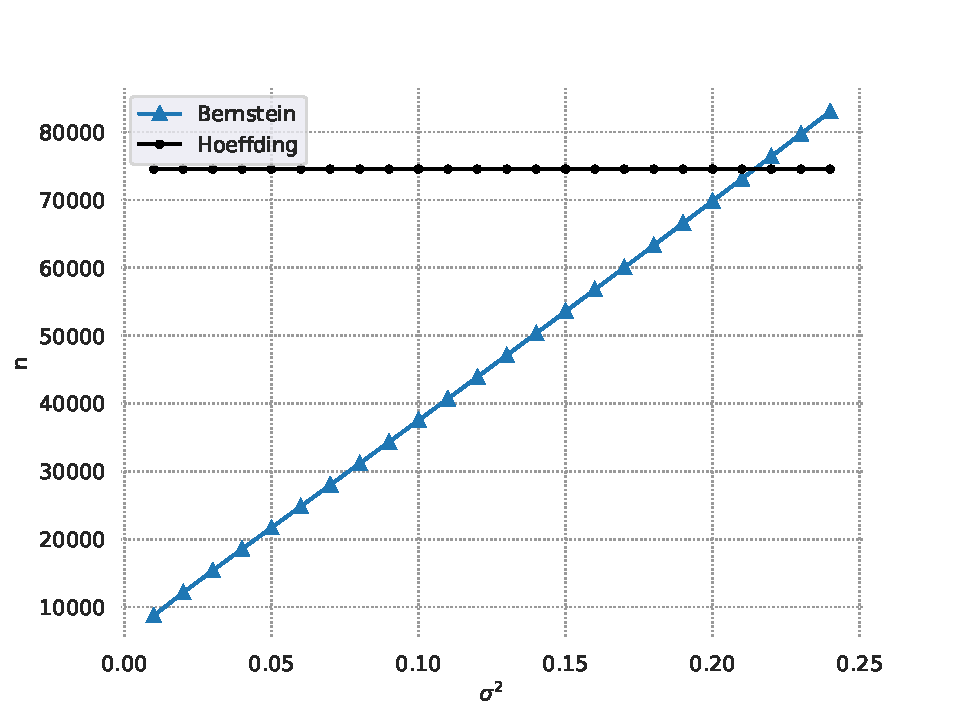
\includegraphics[width=0.75\textwidth]{imagens/t_eq_n.pdf}
		%latinmodern w pythonie
		\caption{Wykres maksymalnej potrzebnej liczby testów w zależności od wariancji zmiennych losowych  $X_i$ w przypadku, gdy liczba przeprowadzonych testów jest równa liczbie gier ($t = n$) dla $\epsilon=0,01$ i $\delta = 0,05$.}
		\label{fig:t_eq_n}
	\end{figure}
	Z rysunku \ref{fig:t_eq_n} widzimy, że algorytm oparty o nierówność Bernsteina szybciej kończy działanie w przypadku, gdy jedna z porównywanych strategii jest silnie dominująca. Co więcej, z równania \eqref{eq:ILEBR Hoeffdin} wynika, że niezależnie od liczby wykonywanych testów, dla $\delta_n = \frac{0,05}{74540}$ maksymalna liczba gier, po której z prawdopodobieństwem $1-0,05$ wiemy, że $|\overline{X_i} - \mu| \le 0,01$ wynosi $74540$. 
	
	Algorytm \ref{alg:ILEBR 1} jest modyfikacją algorytmu \ref{alg:LEBR} na stronie \pageref{alg:LEBR} uwzględniającą ograniczenie, na maksymalną liczbę wykonywanych testów, wynikające z analizy nierówności Bernsteina i Hoeffdinga. W szczególności został dodany warunek zatrzymania algorytmu, gdy liczba wykonanych testów przekroczy $\nmax$. 
	\begin{polishalgorithm}\captionsetup{labelformat=custom}
		\caption{ILEBR 1}\label{alg:ILEBR 1}
		\footnotesize\begin{algorithmic}
			\Ensure \precision $\epsilon$, \probability $\delta$
			\State $LB \gets 0, \quad UB \gets \infty, \quad t \gets 0, \quad n \gets 1$
			\State \find $\nmax$ \suchas $		\epsilon =  \sqrt{\frac{\ln(2\nmax/\delta)}{2\nmax}} $
			\Statex $\delta_n = \delta/\nmax$
			\While{$ UB - LB > 2\epsilon $ \algor $n\le \nmax$}  
			\State $t \gets t + 1$
			\State \obtain $X_t$
			\State $\epsilon_n \gets \overline{\sigma}_n \sqrt{\frac{2\ln(3/\delta_n)}{n}} + \frac{3  \ln{(3 / \delta_n)}}{n}$ 
			\State $LB \gets \max(LB, \overline{X_n} - \epsilon_n)$
			\State $UB \gets \min(UB, \overline{X_n} + \epsilon_n)$
			\State $n \gets n + 1$
			\EndWhile
			\State \Return $ \overline{X_t}$		
		\end{algorithmic}
	\end{polishalgorithm}
	\section{Algorytm ILEBR 2}
	Algorytmy \ref{alg:LEBR} na 
	 \pageref{alg:LEBR} oraz algorytmy \ref{alg:ILEBR 1} na stronie \pageref{alg:ILEBR 1} przeprowadzały testy po każdej rozegranej grze, co skutkuje wystąpieniem bardzo dużej liczby testów. Wprowadźmy pewną zmianę do naszych algorytmów. Zamiast przeprowadzać test po każdej rozegranej grze, niech test odbywa się w momencie, gdy liczba rozegranych gier będzie równa wartości pewnej funkcji zależnej od liczby przeprowadzonych testów. Na podstawie wyników z~artykułu autorstwa Heidricha~Meisnera wiemy, że funkcją, która pozwoli nam na polepszenie wyników jest $t = n^2$~\cite{heidrich2011non}. Aby uzyskać optymalne wyniki, przeprowadźmy tę samą procedurę, jak w przypadku wyrażeń \eqref{eq:ILEBR Hoeffdin} i~\eqref{eq:ILEBR Bernstein}, ale zamiast stosować $t = n$ w~lematach \ref{Hoeffding ineq lemma} i \ref{Bernsteina emp ineq lemma} zastosujemy $t = n^2$.
	
	W przypadku granicy opartej o nierówność Hoeffdinga otrzymujemy
	\begin{gather}
		\label{eq:ILEBR Hoeffdin t=n^2}
		0,01 \le \sqrt{\frac{\ln(2\nmax/\delta)}{2\nmax^2}} \implies \tmax = \lceil \nmax \rceil^2 = \lceil213\rceil^2= 45369.
	\end{gather}

	W przypadku granicy opartej o nierówność Bernsteina otrzymujemy
	\begin{gather}
		\label{eq:ILEBR Bernstein t=n^2_1}
		0,01 \le \sqrt{\frac{\ln(\frac{3\nmax}{0,05})}{\nmax^2}} + \frac{3  \ln(\frac{3\nmax}{0,05})}{\nmax^2}\implies \tmax = \lceil \nmax \rceil^2 = \lceil230,751^2\rceil= 53247. 
	\end{gather}
	\begin{figure}
		\centering
		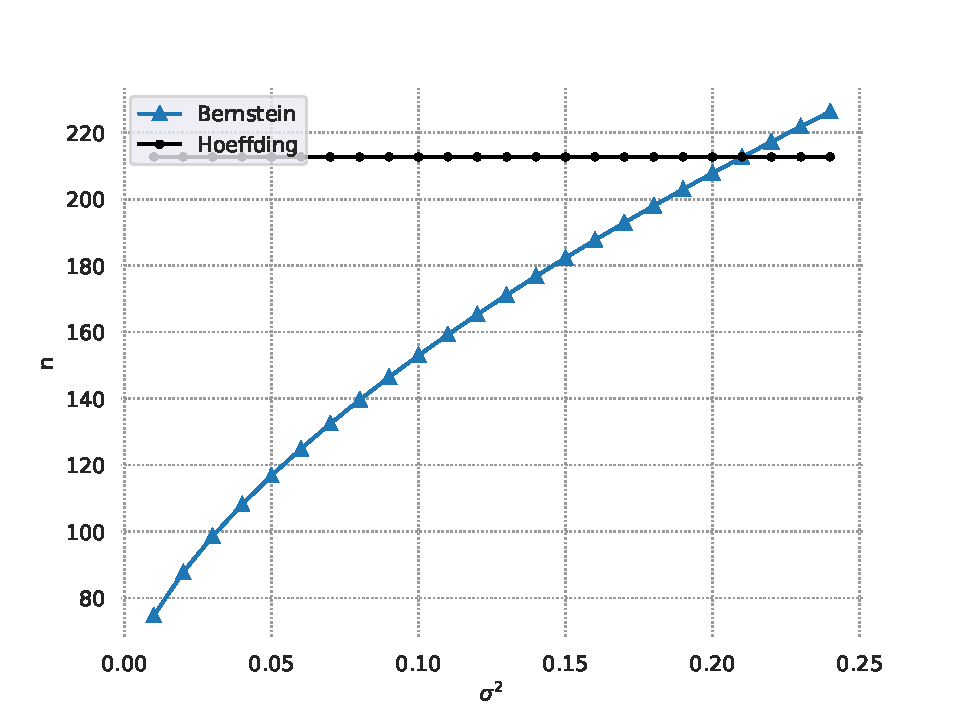
\includegraphics[width=0.80\textwidth]{imagens/t_eq_n_q.pdf}
%		\captionsetup{justification=centering}
		\caption{Wykres maksymalnej potrzebnej liczby testów w zależności od wariancji zmiennych losowych  $X_i$ w przypadku, gdy liczba rozegranych gier jest równa liczbie przeprowadzonych testów do kwadratu  dla $\epsilon=0,01$ i $\delta = 0,05$.}
		\label{fig:t_eq_n_q}
	\end{figure}
	Porównując uzyskane wartości \eqref{eq:ILEBR Hoeffdin t=n^2}, \eqref{eq:ILEBR Bernstein t=n^2_1} z wartościami \eqref{eq:ILEBR Hoeffdin} i \eqref{eq:ILEBR Bernstein}, widzimy, że udało się nam zmniejszyć maksymalną liczbę gier, które należy wykonać z 74540 do 45369. Wprowadźmy więc nowe poprawki do algorytmu \ref{alg:ILEBR 2}.
	\begin{polishalgorithm}\captionsetup{labelformat=custom}
		\caption{ILEBR 2}\label{alg:ILEBR 2}
		\footnotesize\begin{algorithmic}
			\Ensure \precision $\epsilon$, \probability $\delta$
			\State $LB \gets 0, \quad UB \gets \infty, \quad t \gets 0, \quad n \gets 1$
			\State \find $\nmax$ \suchas $		\epsilon =  \sqrt{\frac{\ln(2\nmax/\delta)}{2\nmax^2}} $
			\Statex $\delta_n = \delta/\nmax$
			\While{$ UB - LB > 2\epsilon $ \algor $n \le \nmax$}  
			\While{$t \le n^2$}
			\State $t \gets t + 1$
			\State \obtain $X_t$
			\EndWhile
			\State $\epsilon_n \gets \overline{\sigma}_n \sqrt{\frac{2\ln(3/\delta_n)}{n^2}} + \frac{3  \ln{(3 / \delta_n)}}{n^2}$ 
			\State $LB \gets \max(LB, \overline{X_n} - \epsilon_n)$
			\State $UB \gets \min(UB, \overline{X_n} + \epsilon_n)$
			\State $n \gets n + 1$
			\EndWhile
			\State \Return $ \overline{X_t}$		
		\end{algorithmic}
	\end{polishalgorithm}
	\section{Algorytm ILEBR*}
	Do tej pory wszystkie stosowane algorytmy wyznaczały nam prawdopodobieństwo wygranej pierwszego gracza. Jednak nam nie zależy na tym, aby dokładnie oszacować prawdopodobieństwo wygranej. Głównym celem algorytmów jest wyznaczenie lepszej strategii. Pozwala nam to na zaproponowanie modyfikacje algorytmu \ref{alg:ILEBR 2} o nowe warunki zatrzymania. Warunkiem tym jest zatrzymanie działania algorytmu w momencie, gdy górna bądź dolna granica przekroczy wartość $0,5$. 
	\begin{polishalgorithm}\captionsetup{labelformat=custom}
		\caption{ILEBR* 1}\label{alg:IEBLR* 1}
		\footnotesize\begin{algorithmic}
			\Ensure \precision $\epsilon$, \probability $\delta$ 
			\State  $ LB \gets 0,\quad UB \gets \infty,\quad t \gets 1,\quad n \gets 0 $
			\State \find $\nmax$ \suchas $		\epsilon =  \sqrt{\frac{\ln(2\nmax/\delta)}{2\nmax^2}} $
			\Statex $\delta_n = \delta/\nmax$
			\While{$( UB - LB > 2\epsilon $ \algor $n \le \nmax)$ \algand $ (UB > 0,5 \text{ \algor } LB < 0,5)$}
			\While{$t \le n^2$} 
			\State $t \gets t + 1$
			\State \obtain $X_t$
			\EndWhile 
			\State $\epsilon_n \gets \overline{\sigma}_n \sqrt{\frac{2\ln(3/\delta_n)}{n^2}} + \frac{3  \ln{(3 / \delta_n)}}{n^2}$ 
			\State $LB \gets \max(LB,  \overline{X_n} - \epsilon_n)$
			\State $UB \gets \min(UB,  \overline{X_n} + \epsilon_n)$
			\State $n \gets n + 1$
			\EndWhile
			\If{$LB > 0,5$}
			\State \Return $p_1$ \win
			\ElsIf{$UB < 0,5$}
			\State \Return $p_2$ \win
			\ElsIf{$\overline{X_n} > 0,5$}
			\State \Return $p_1$ \win
			\Else
			\State \Return $p_2$ \win
			\EndIf
		\end{algorithmic}
	\end{polishalgorithm}
	\section{Algorytm ILEBR* 2}
	Do tej pory skupialiśmy się na ograniczeniu maksymalnej liczby rozgrywanych gier. Jednak oczywiste jest, że nie ma sensu testować, który z graczy jest lepszy, gdy liczba rozegranych gier jest zbyt mała. 
	
	Zajmijmy się wyznaczeniem minimalnego $t$, po którym przeprowadzamy pierwszy test. Algorytm oparty na nierówności Bernsteina najszybciej wyznacza wynik, gdy wariancja naszej zmiennej losowej wynosi 0.
	Interesuje nas moment, od którego będziemy w stanie rozróżnić, kiedy dolna lub górna granica przekroczy $0,5$. Korzystając z lematu \ref{Bernsteina emp ineq lemma} dla $\overline{\sigma}_t=0$, $t = n^2$ i $\nmax = 213$ możemy oszacować 
	\begin{gather*}
		\label{eq:ILEBR Bernstein t=n^2}
		0,5 \le \frac{3  \ln(\frac{3 \cdot213}{0,05})}{n_{min}^2}\implies \tmin = \lceil \nmin \rceil^2 = \lceil 7,53219 \rceil^2= 64. 
	\end{gather*}
	Oznacza to, że przy $\epsilon = 0,01$ i $\delta = 0,05$ w przypadku, gdy jeden gracz zawsze wygrywa, będziemy w stanie to stwierdzić nie wcześniej niż po rozegraniu $64$ gier.
	Na tej podstawie wyznaczmy nowe $\nmax$ uwzględniając pomijanie pierwszych niepotrzebnych testów.
	\begin{gather}
		\label{eq:ILEBR Hoeffdin t=n^2 and t_min}
		0,01 \le \sqrt{\frac{\ln(2\nmax/0,05)}{2(\nmax+7)^2}} \implies \tmax = \lceil \nmax+7\rceil^2 = \left\lceil 205,289+7\right\rceil^2= 45369.
	\end{gather}
	Chociaż wynik równania \eqref{eq:ILEBR Hoeffdin t=n^2 and t_min} nie zmniejszył maksymalnej liczby testów jakie należy wykonać, to pozwolił nam on na zmniejszenie $\epsilon_n$. Oznacza to, że stosując odroczenie pierwszych testów, możemy dokładniej oszacować naszą górną i dolną granicę.
	\begin{polishalgorithm}[H]\captionsetup{labelformat=custom}
		\caption{ILEBR* 2}\label{alg:IEBLR* 2}
		\footnotesize\begin{algorithmic}
			\Ensure \precision $\epsilon$, \probability $\delta$ 
			\State  $ LB \gets 0,\quad UB \gets \infty, \quad n \gets 0 $
			\State \find $\nmax$ \suchas $		\epsilon =  \sqrt{\frac{\ln(2\nmax/\delta)}{2\nmax^2}} $
			\State \find $\nmin$ \suchas $		0,5 =  \sqrt{\frac{\ln(2\nmax/\delta)}{2(\nmin+1)^2}} $
			\State \obtainfirstgames{$X_1, X_2, X_{\nmin}$}  
			\State $t \gets \nmin^2$
			\Statex $\delta_n = \delta/\nmax$
			\While{$( UB - LB > 2\epsilon $ \algor $n \le \nmax)$ \algand $ (UB > 0,5 \text{ \algor } LB < 0,5)$}
			\While{$t \le (n+\nmin)^2$} 
			\State $t \gets t + 1$
			\State \obtain $X_t$
			\EndWhile
			\State $\epsilon_n \gets \overline{\sigma}_n \sqrt{\frac{2\ln(3/\delta_n)}{(n+\nmin)^2}} + \frac{3  \ln{(3 / \delta_n)}}{(n+\nmin)^2}$ 
			\State $LB \gets \max(LB,  \overline{X_n} - \epsilon_n)$
			\State $UB \gets \min(UB,  \overline{X_n} + \epsilon_n)$
			\State $n \gets n + 1$
			\EndWhile
			\If{$LB > 0,5$}
			\State \Return $p_1$ \win
			\ElsIf{$UB < 0,5$}
			\State \Return $p_2$ \win
			\ElsIf{$\overline{X_n} > 0,5$}
			\State \Return $p_1$ \win
			\Else
			\State \Return $p_2$ \win
			\EndIf
		\end{algorithmic}
	\end{polishalgorithm}

	\section{Prawdopodobieństwo popełnienia błędu}
		Algorytmy typu LEBR charakteryzują się odmiennym prawdopodobieństwem popełnienia błędu niż klasyczne algorytmy racingowe. Wynika to z wprowadzenia parametru~$\epsilon$.
		
		W tej sekcji zajmiemy się określeniem tego prawdopodobieństwa w zależności od parametrów początkowych $\delta$ i $\epsilon$ w badanym problemie decyzyjnym. W tym celu zaproponujemy dwie hipotezy dotyczące graczy:
	\begin{itemize}
		\item $\text{H}_a$ \pauza Gracz pierwszy jest lepszy od gracza drugiego;
		\item  $\text{H}_b$ \pauza Gracz pierwszy jest gorszy od gracza drugiego.
	\end{itemize}
	To oznacza, że prawdopodobieństwem popełnienia błędu w naszym przypadku jest prawdopodobieństwo uznania za lepszego gracza osoby o mniejszym prawdopodobieństwie zwycięstwa.
	
	Oznaczmy prawdopodobieństwo pomyłki w naszych algorytmach typu LEBR jako $\alpha$. Bez straty ogólności załóżmy, że teoretyczne prawdopodobieństwo wygrania gry przez pierwszego gracza jest większe od $0,5$ ($\mu > 0,5$)%!czy usunac to wtracenie
	. Wtedy prawdopodobieństwo $\alpha$ możemy wyrazić za pomocą następującego wzoru
	\begin{gather}
		\label{eq:error probability}
		\alpha = 1 - \probP_{\mu}(\overline{X}_{f(\nmax)} > 0,5)
 \prod^{\nmax}_{k=1} \probP_{\mu}(\overline{X}_{f(k)} +  \epsilon_{k} > 0,5),
	\end{gather}
	gdzie:
	\begin{itemize}
		\item $\alpha$ \pauza Prawdopodobieństwo popełnienia błędu;
		\item $f(k)$ \pauza Funkcja rozmiaru próby, zależna od liczby przeprowadzonych testów;
		\item $\epsilon_k = \overline{\sigma}_k \sqrt{\frac{2\ln(3/\delta_k)}{f(k)}}+\frac{3\ln(3/\delta_k)}{f(k)}$ \pauza Zależny od testowanego algorytmu;
		\item $\nmax$ \pauza Zależny od przyjętych parametrów $\epsilon$ i $\delta$.
	\end{itemize}
	Dowód wyrażenia \eqref{eq:error probability} znajduje się na końcu niniejszej pracy w dodatku \ref{proof:error probability}.
	
	Wyrażenie \eqref{eq:error probability} pozwala nam określić teoretyczne prawdopodobieństwo wystąpienia błędu dla algorytmów typu LEBR. Niestety, wzór ten nie umożliwia nam na łatwe wyznaczenie takiej wartości parametru $\delta$, aby prawdopodobieństwo błędu było mniejsze niż żądane $\alpha$. Aby uzyskać metodę wyznaczania takiej $\delta$ dla zadanego parametru początkowego~$\epsilon$, ograniczmy z góry prawdopodobieństwo błędu $\alpha$ wynikające z równania \eqref{eq:error probability}.
	\begin{gather}
		\label{eq:error_probability_limit_1}
		\alpha \le
		  1-\prod^{\nmax}_{k=1} \probP_{\mu}(\overline{X}_{f(k)} +  \epsilon_{k} > 0,5) +
		 \probP_{\mu}(\overline{X}_{f(\nmax)}\le 0,5).
	\end{gather}
	\noindent
	Wyrażenie \eqref{eq:error_probability_limit_1} możemy zapisać przy pomocy dwóch składników. Pierwszym z nich jest 
	\begin{gather}
		\alpha_1 = \label{eq:error_a1}
		\probP_{\mu}(\overline{X}_{f(\nmax)} \le 0,5),
	\end{gather}
	drogim natomiast
	\begin{gather}
		\label{eq:error_a2}
		\alpha_2 = 1 - \prod^{\nmax}_{k=1} \probP_{\mu}(\overline{X}_{f(k)} +  \epsilon_{k} > 0,5).
	\end{gather}
	Zakładając, że $X_i$ jest zmienną losową z rozkładu zero-jedynkowego, możemy stwierdzić, że $Y_n = \sum_{i=1}^{n}X_i$ jest zmienną losową o rozkładzie dwumianowym. To pozwala nam zapisać równania \eqref{eq:error_a1} i \eqref{eq:error_a2} w następujący sposób:
	\begin{gather}
		\label{eq:error_a1_1}
		\alpha_1 = \probP_{\mu}\left( Y_{f(\nmax)} \le  \frac{f(\nmax)}{2} \right),\nonumber \\
		\label{eq:error_a2_1}
		\alpha_2 = 1 - \prod_{k=1}^{\nmax} \probP_{\mu}\left( Y_{f(\nmax)}  > \frac{f(k)}{2} - \overline{\sigma}_{f(k)} \sqrt{2\ln(3/\delta_k)f(k)} - 3  \ln{(3 / \delta_k)} \right).
	\end{gather}
	
	Analizując rysunek \ref{fig:a2_probability} oraz wyrażenie \eqref{eq:error_a2_1} możemy zauważyć, że maksymalne $\alpha_2$ jest osiągane dla $\mu = 0,5$, zatem
	\begin{align}
		\label{eq:errpr_a2_limit_1}
		\alpha_2 \le 1 - \prod_{k=1}^{\nmax} \probP_{0,5}\left( Y_{f(\nmax)}  > \frac{f(k)}{2} -  \sqrt{\frac{\ln(3/\delta_k)f(k)}{2}} - 3  \ln{(3 / \delta_k)} \right).
	\end{align}
	Nierówność \eqref{eq:errpr_a2_limit_1} możemy jeszcze bardziej ograniczyć ze względu na fakt, że $\delta\in(0, 1]$. Analizując rysunek \ref{fig:a2_probability} i nierówność \eqref{eq:errpr_a2_limit_1}, możemy zauważyć, że wartość prawdopodobieństwa $\alpha_2$ rośnie wraz ze wzrostem parametru $\delta$. Oznacza to, że możemy zwiększyć nasze ograniczenie, zastępując $\delta_n = \delta/\nmax$ samym $1/\nmax$.
	\begin{align}
		\label{eq:errpr_a2_limit_2}
		\alpha_2 \le 1 - \prod_{k=1}^{\nmax} P_{0,5}\left( Y_{f(\nmax)}  > \frac{f(k)}{2} -  \sqrt{\frac{\ln(3\nmax)f(k)}{2}} - 3  \ln{(3\nmax})  \right).
	\end{align}
	\noindent
	Wynik uzyskany z nierówności \eqref{eq:errpr_a2_limit_2} jest szczególnie istotny, ponieważ ograniczenie to zależny jawnie tylko od parametru $\nmax$.

	W celach uproszenia zapisy wprowadźmy funkcję  $F'_{\mu}(\nmax)$ zdefiniowaną następująco:
	\begin{gather}
		F'_{\alpha_1}(\nmax) = P_{\mu}\left( Y_{f(\nmax)}  \le \frac{f(\nmax)}{2} \right),\nonumber \\
		F'_{\alpha_2}(\nmax) = 1 - \prod_{k=1}^{\nmax} P_{0,5}\left( Y_{f(k)}  > \frac{f(k)}{2} - \sqrt{\frac{\ln(3\nmax)}{2}f(k)} - 3  \ln{(3 \nmax)}\right),\nonumber \\
		\label{eq:error_a_limit}
		F'_{\mu}(\nmax) =  F'_{\alpha_1}(\nmax)+F'_{\alpha_2}(\nmax).
	\end{gather}
		Łącząc wyniki uzyskane z
		\eqref{eq:error_probability_limit_1} i \eqref{eq:error_a_limit} otrzymujemy, że dla $\mu > 0,5$
	\begin{gather}
		\label{eq:error_a_limit_end}
		F'_{\mu}(\nmax) \ge \alpha .
	\end{gather}
		Ze względu na symetrie rozważanego problemu, nierówność \eqref{eq:error_a_limit_end} możemy zapisać dla dowolnego $\mu$ w następujący sposób
	\begin{align}
		\label{eq:F_function}
		F_{\mu}(\nmax) = 
		\begin{cases}
			F'_{1-\mu}(\nmax), &\text{dla }  \mu\le0,5,\\
			F'_{\mu}(\nmax), &\text{dla } \mu>0,5.
		\end{cases}
	\end{align}
	\noindent
	Funkcja \eqref{eq:F_function} pozwala nam na określenie prawdopodobieństwa popełnienia błędu dla algorytmów typu LEBR. Ponadto, przy zadanej wartości początkowej parametru $\epsilon$ możemy dobrać wartość $\delta$ tak, aby nierówność $F_{\mu}(\nmax) \ge \alpha$ była spełniona. Takie $\delta$ możemy wyznaczyć poprzez znalezienie rozwiązania układu równań
	\begin{gather}
		\label{eq:alpfa_determinant}
		\left\{
		\begin{split}
			\nmax =& \min \left\{n\in \mathbb{N}^+: F_{\mu}(n) < \alpha \right\}, \\
			\delta =&\cfrac{2\nmax}{\exp(2\epsilon^2f(\nmax))}.
		\end{split}
		\right. 
	\end{gather}
	Dowód wyrażenia \eqref{eq:alpfa_determinant} znajduje się na końcu niniejszej pracy w dodatku \ref{proof:alpfa_determinant}.
	
	W ramach sprawdzenia wyznaczmy prawdopodobieństwo wyznaczenia złego gracza dla Algorytmu ILEBR* i parametrów początkowych $\mu = 0,497, \delta=0,05, \epsilon=0,01$.
	Wtedy:
	\begin{gather}
		\label{eq:error preparation}
		\nmax = 213,\quad
		 \epsilon_n = \overline{\sigma}_n \sqrt{\frac{2\ln(3/\delta_n)}{n^2}} + \frac{3  \ln{(3 / \delta_n)}}{n^2},\quad
		  f(n) = n^2,\quad 
		  \delta_n = \frac{\delta}{\nmax}.
	\end{gather}
	Podstawiając \eqref{eq:error preparation} do \eqref{eq:F_function} otrzymujemy, że
	\begin{gather}
		\label{eq:alpha_result}
		F_{0,497}(213)  \approx 0,10083 \ge \alpha.
	\end{gather}
	\noindent
	Wynik \eqref{eq:alpha_result} zgadza się z wynikami symulacji dla algorytmu ILEBR* przedstawionymi na rysunku \ref{fig:test_powrs} na stronie \pageref{fig:test_powrs}.
	Co więcej, możemy również wyznaczyć wartość parametru $\delta$ tak, aby $F_{0,497}(\nmax) \le 0,05$. Aby to osiągnąć, znajdziemy $\nmax$ i $\delta$ spełniające zależność~\eqref{eq:alpfa_determinant} przy ustalonym $\epsilon = 0,01$ i $\alpha=0,05$.
	Rozwiązaniem tego problemu przy zadanych parametrach początkowych jest $\nmax = 293, \delta = 2,047143\cdot10^{-5}$. Rysunek \ref{fig:test_powrs_alpha_0_05} na stronie~\pageref{fig:test_powrs_alpha_0_05} przedstawia zgodność symulacji z naszymi teoretycznymi rozważaniami.
	\begin{figure}
		\centering
		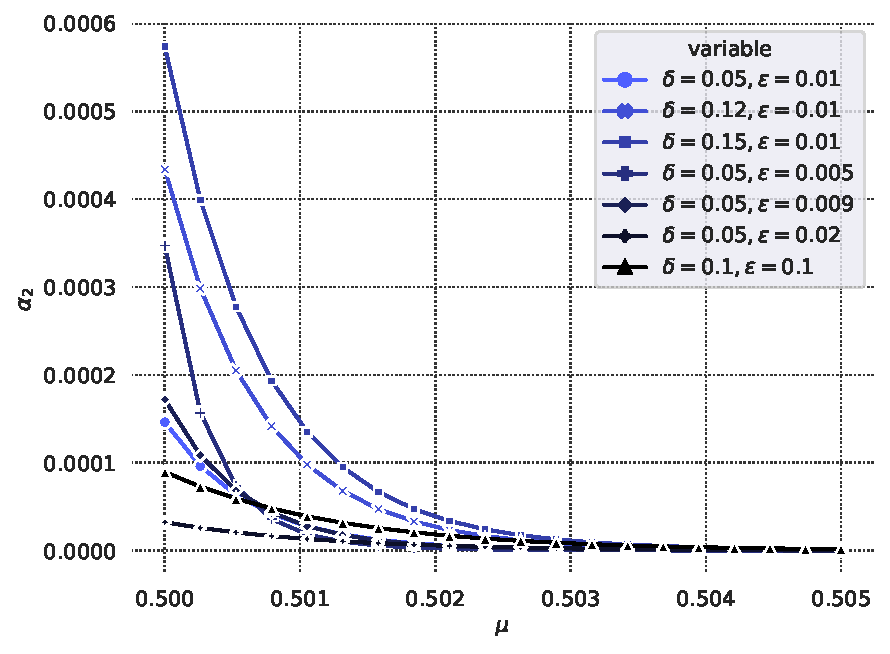
\includegraphics[width=0.8\textwidth]{imagens/alpha_2.pdf}
		%		\captionsetup{justification=centering}
		\caption{Wykres wartości prawdopodobieństwa $\alpha_2$ w zależności od $\mu$, $\delta$ i $\epsilon$ dla algorytmu ILEBR*.}
		\label{fig:a2_probability}
	\end{figure}

	\begin{figure}
		\centering
		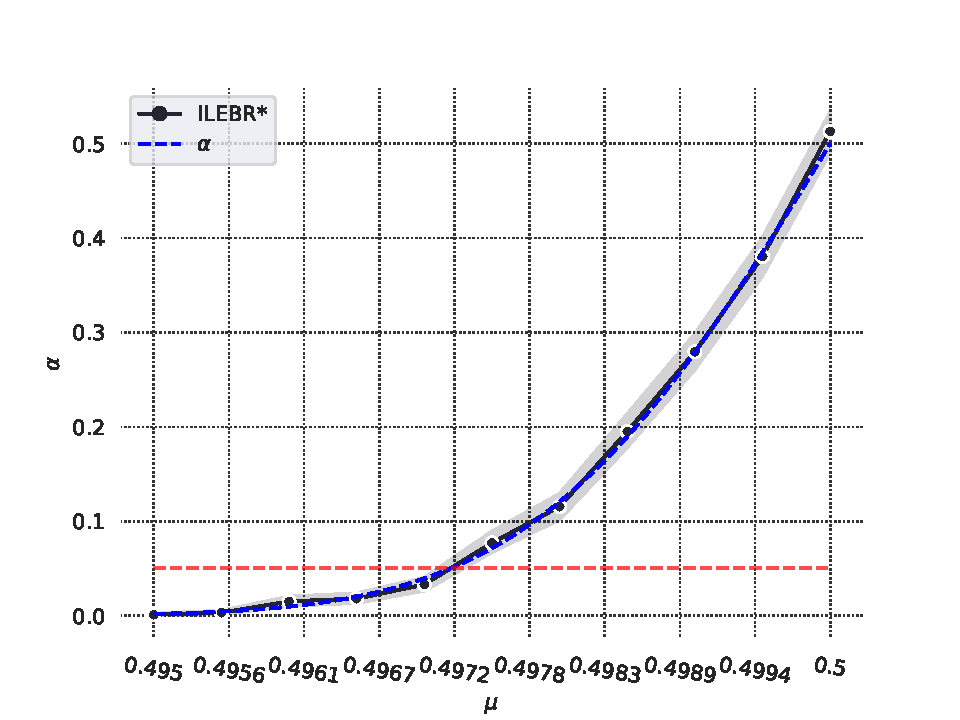
\includegraphics[width=0.8\textwidth]{imagens/test_powrs_alpha_0_05.pdf}
		%		\captionsetup{justification=centering}
		\caption{Wykres wartości prawdopodobieństwa $\alpha$ w zależności od $\mu$ dla $\epsilon =0,01$, $\delta =2,047143\cdot10^{-5}$ i algorytmu ILEBR*.}
		\label{fig:test_powrs_alpha_0_05}
	\end{figure}
	%zamiast pisac test statystyczzny uzywac problem decyzyjny
	%zamiast mocy prawdopodobienstwo błędu
	\begin{figure}
		\centering
		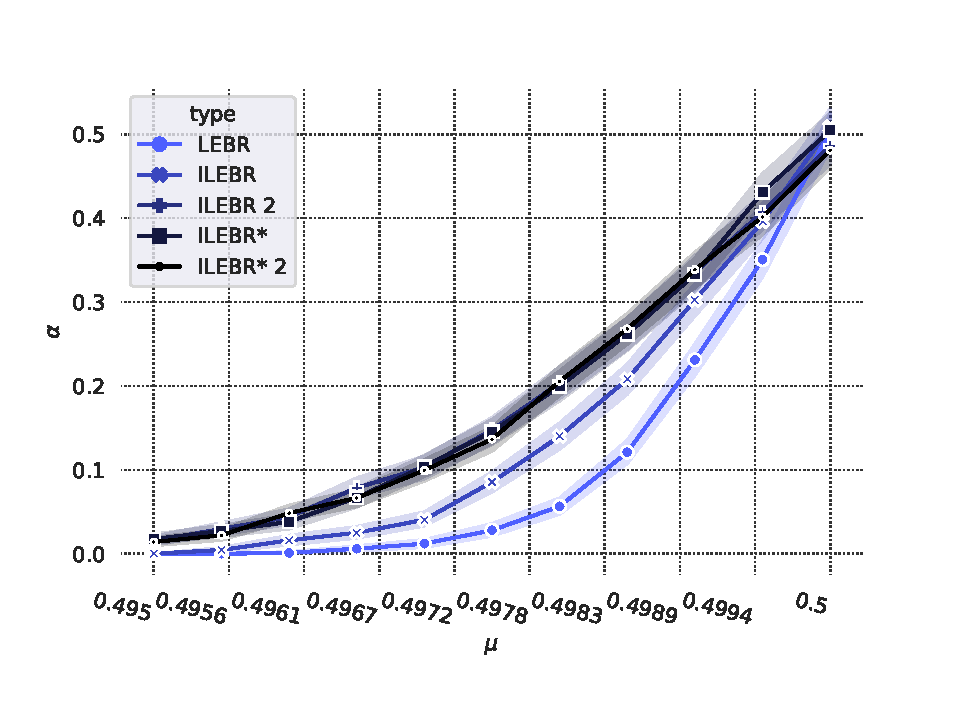
\includegraphics[width=0.8\textwidth]{imagens/test_powrs.pdf}
		\caption{Wykres wartości prawdopodobieństwa $\alpha$ dla porównywanych algorytmów, w~zależności od $\mu$ dla $\epsilon = 0,01$ i $\delta = 0,05$.}
		\label{fig:test_powrs}
	\end{figure}
	\begin{figure}
		\centering
		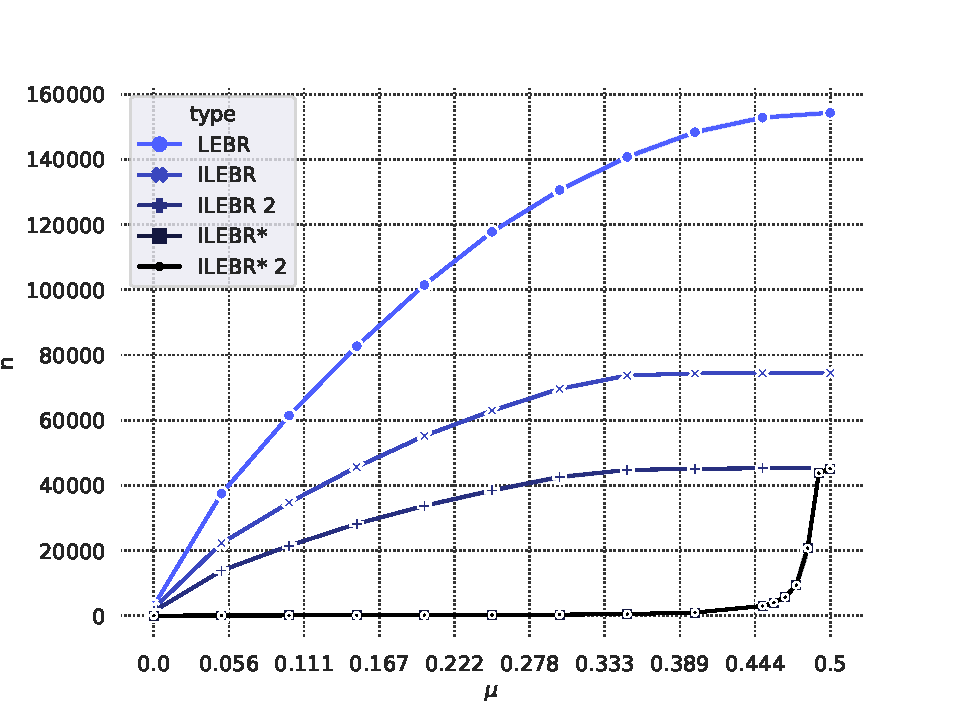
\includegraphics[width=0.8\textwidth]{imagens/needed_games_to_play.pdf}
		\caption{Wykres średniej liczby gier potrzebnych do rozegrania w zależności od wartości oczekiwanej zmiennych losowych $X_i$ dla $\epsilon=0,01$ i $\delta = 0,05$. Na wykresie widoczne są 4~krzywe, ponieważ wyniki dla algorytmów ILEBR* i ILEBR* 2 pokrywają się ze sobą.}
		\label{fig:needed_games_to_play}
	\end{figure}
	\begin{figure}
		\captionsetup[subfigure]{width=0.8\textwidth}
		\centering
		\begin{subfigure}{0.8\textwidth}
			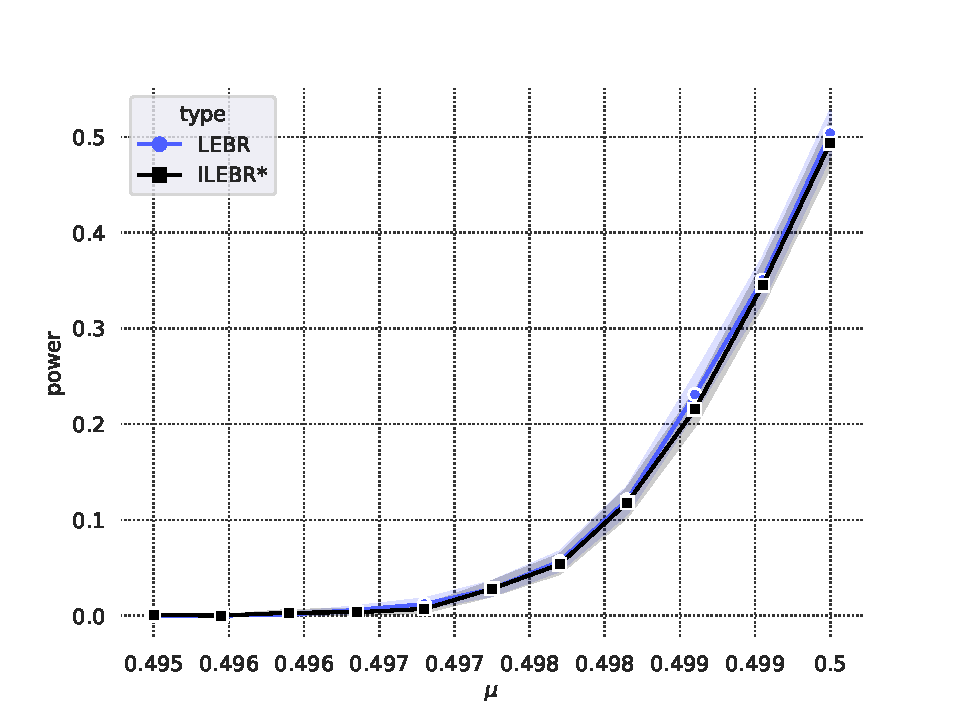
\includegraphics[width=1\linewidth]{imagens/test_powrs_same_n_max.pdf}
			\caption{Wykres prawdopodobieństwa pomyłki w zależności od $\mu$ dla $\epsilon=0,01$.}
			\label{fig:power_same_n_max}
		\end{subfigure}
		\begin{subfigure}{.5\textwidth}
			\centering
			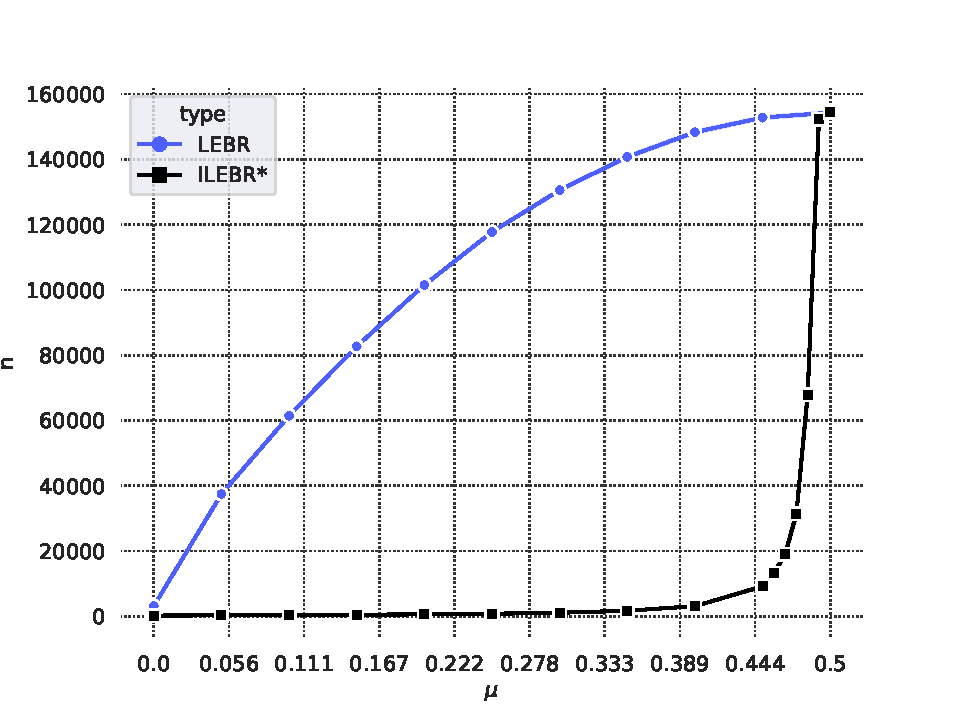
\includegraphics[width=1\linewidth]{imagens/needed_games_to_play_same_n_max.pdf}
			\caption{Wykres średniej liczby gier potrzebnej do rozegrania w zależności od $\mu$ dla $\epsilon=0,01$.}
			\label{fig:power_same_n_max_log}
		\end{subfigure}%
		\begin{subfigure}[r]{.5\textwidth}
			\centering
			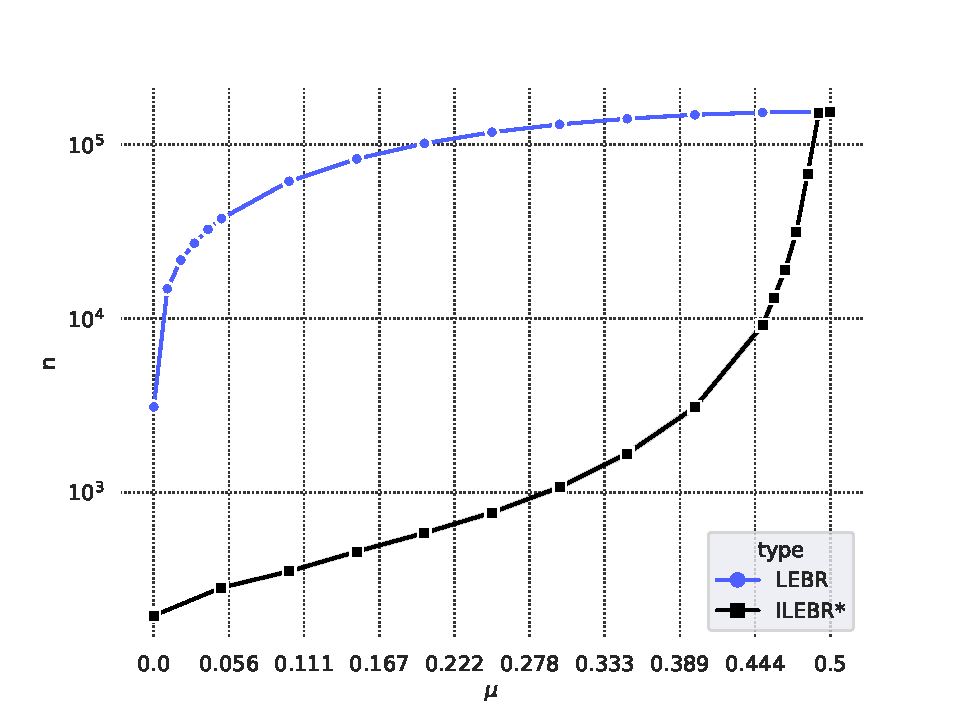
\includegraphics[width=1\linewidth]{imagens/needed_games_to_play_same_n_max_log.pdf}
			\caption{Wykres średniej liczby gier potrzebnej do rozegrania w zależności od $\mu$ dla $\epsilon=0,01$ w skali logarytmicznej.}
			\label{fig:game_to_play_same_n_max}
		\end{subfigure}
		\caption{Porwanie algorytmów LEBR oraz ILEBR* w przypadku, gdy średnie $\nmax$ są sobie równe.}
		\label{fig:same_n_max}
	\end{figure}
	Spoglądając na rysunek \ref{fig:test_powrs} na stronie \pageref{fig:test_powrs} widzimy, że wszystkie testy charakteryzują się niskim prawdopodobieństwem popełnienia błędu i sprawdzają się dobrze, dopóki prawdopodobieństwo wygranej jednego z graczy nie przekroczy $0,495$ przy zadanych wartościach parametrach początkowych. Obszary ściemnione oznaczają przedziały ufności o współczynniku ufności 95\%.
	
	Porównując ze sobą wyniki przedstawione na rysunki \ref{fig:test_powrs} i \ref{fig:needed_games_to_play} na stronie  \pageref{fig:needed_games_to_play} możemy zauważyć, że algorytm LEBR charakteryzuje się najniższym prawdopodobieństwem popełnienia błędu wśród badanych metod.
%	 Wynika to jednak z dużej wielkości próby, która jest wykorzystywana w tym algorytmie.	
	Jednak by osiągnąć taki rezultat, algorytm ten wymaga użycia większej liczby gier, niż pozostałe testowane metody.
	
	Test statystyczny oparty o algorytm ILEBR ma większe prawdopodobieństwo popełnienia błędu, ale pozwala nam na prawie dwukrotnie zmniejszenie liczby wymaganych gier. Dodatkowo widzimy, że algorytmy  ILEBR 2, ILEBR* i ILEBR* 2 cechują się takim samym prawdopodobieństwem pomyłki, jednak wersje algorytmów oznaczone (*) pozwalają nam na ograniczenie liczby gier potrzebnej do rozegrania, aby test mógł wyznaczyć lepszego gracza. W poniższej pracy będziemy stosować algorytm ILEBR* 2, ponieważ pozwoli on nam na znaczne zmniejszenie liczby porównań, jakie będziemy przeprowadzać w celu wyznaczenia lepszego gracza. 
	
	Jeśli jednak stanowi dla nas problem, że algorytmy oznaczone (*) charakteryzują się większym prawdopodobieństwem popełnienia błędu w porównaniu do algorytmu LEBR przy takich samych parametrach początkowych, to możemy łatwo osiągnąć takie samo prawdopodobieństwo, wystarczy, aby $\nmax$ w obu tych algorytmach były sobie równe.
	Analizując rysunek~\ref{fig:same_n_max} na stronie \pageref{fig:same_n_max} widzimy, że przy zachowaniu tego samego prawdopodobieństwa pomyłki, algorytm ILEBR* jest znacznie szybszy niż jego oryginalny odpowiednik. W naszym przypadku algorytm ILEBR* z parametrami początkowymi $\epsilon =0,01, \delta =3,02101484 \cdot 10^{-11}$ zachowuje takie samo prawdopodobieństwo popełnienia błędu jak algorytm LEBR z~parametrami początkowymi $\epsilon=0,01, \delta=0,05$.

	
	
	\chapter{Algorytmy wyznaczania optymalnej strategii}
	Wszystkie algorytmy przedstawione w tym rozdziale są algorytmami genetycznymi \cite{Figielska2006}. 
	Algorytm genetyczny to sposób tworzenia nowych rozwiązań dla danego problemu poprzez iteracyjne stosowanie procesu ewolucyjnego. W tym procesie tworzone są nowe rozwiązania, ocenia się ich jakość i wybierane najlepsze z nich, aby stworzyć kolejną generację rozwiązań. Ten proces powtarza się, aż zostanie znalezione rozwiązanie spełniające określone kryteria. Algorytm generacyjny może być używany do rozwiązywania różnych rodzajów problemów, takich jak optymalizacja, uczenie maszynowe, tworzenie sztucznej inteligencji i wiele innych. Algorytmy ewolucyjne są często interpretowane jako odwzorowanie procesu ewolucyjnego w naturze, ze względu na swoje upodobnienie do procesu selekcji naturalnej, w którym najlepsze jednostki są wybierane do reprodukcji i tworzenia nowych pokoleń.
	
	Ogólnie rzecz biorąc, algorytm generacyjny składa się z kilku kluczowych kroków:
	\begin{itemize}
		\item Inicjalizacja \pauza Tworzenie początkowego zbioru rozwiązań dla danego problemu;
		\item Ocena \pauza Ocena jakości każdego z rozwiązań za pomocą odpowiedniej funkcji wypłaty lub innych miar;
		\item Selekcja \pauza Wybieranie najlepszych rozwiązań do następnej generacji;
		\item Krzyżowanie \pauza Łączenie najlepszych rozwiązań z poprzedniej generacji, aby stworzyć nowe rozwiązania dla następnej generacji;
		\item Mutacja \pauza Losowa zmiana jednego lub więcej elementów w nowych rozwiązaniach, aby zapewnić różnorodność w następnej generacji;
		\item Powtarzanie \pauza Powtarzanie kroków 2 \ppauza 5, aż zostanie znalezione rozwiązanie spełniające określone kryteria jakości lub osiągnięty zostanie maksymalny poziom iteracji.
	\end{itemize}	
	Proces znajdowania potencjalnych rozwiązań polega na przeszukiwaniu przestrzeni wszystkich możliwych rozwiązań i wybieraniu tych, które dają najlepsze wyniki. W rzeczywistości jednak często nie mamy fizycznej możliwości sprawdzenia wszystkich możliwych rozwiązań lub ich sprawdzenie jest zbyt czasochłonne bądź kosztowne. Dlatego w algorytmach ewolucyjnych często wykorzystuje się techniki probabilistyczne, które pomagają wybierać, tworzyć i wyszukiwać kolejne rozwiązania.
	
	W niniejszej pracy zaprezentujemy 4 algorytmy, których celem jest znalezienie optymalnej strategii. Trzy pierwsze algorytmy zostały opisane na podstawie pracy \cite{cauwet2018surprising}. Czwartym algorytmem jest zaproponowana w niniejszej pracy metoda, jest ona bardzo podobna do algorytmu \ref{alg:Approximate_Coevolution} na stronie \pageref{alg:Approximate_Coevolution}, jednak oparta jest o odmienny sposób rozgrywania gier miedzy graczami. Opis tego algorytmu zostanie przedstawiony w dalszej części pracy.
	\section{Algorytm iteracyjny}
		Pierwszym algorytmem, który zostanie przedstawiony, jest algorytm iteracyjny. Jest to metoda bardzo intuicyjna, opierająca się na stopniowym zwiększaniu skuteczności strategii graczy poprzez porównywanie ich wyników. Gdy znajdziemy strategię, która daje lepsze wyniki niż ta poprzednia, staje się ona nowym punktem odniesienia. Na jej podstawie algorytm będzie kontynuować proces optymalizacji wyników graczy. Nowa strategia jest akceptowana, jeśli wygrywa ona z prawdopodobieństwem większym niż~50\% w~porównaniu do poprzedniej strategii. Algorytm \ref{alg:Iterative} jest przykładem algorytmu ewolucyjnego typu (1+1)~\cite{droste1998rigorous}.
		\begin{polishalgorithm}\captionsetup{labelformat=custom}
			\caption{Algorytm iteracyjny}\label{alg:Iterative}
			\footnotesize\begin{algorithmic}
				\Ensure  \precision $\epsilon$, \probability $\delta$, \randomopponent $x$
				\State $\sigma \gets 1 $ 
				\While{\termination}
				\ForAll{$i = 1$ \tolenghtof x}

				\State $x_i' \gets x_i + \sigma \mathcal{N}(0,1)$ 
				\EndFor
				\While{\bernsteinnotstop}
				\State \playgamebetween $x'$ \algand $x$
				\EndWhile
				\If{$x'$  \betterthen $x$  }
				\State $x \gets x'$
				\State $\sigma \gets 1,25\sigma$
				\Else
				\State $\sigma \gets 0,84 \sigma$
				\EndIf
				\EndWhile
				\State \Return \approximationx 
			\end{algorithmic}
		\end{polishalgorithm}
	\section{Algorytm koewolucyjny}	
	Kolejnym algorytmem ewolucyjnym, którego będziemy używać, jest algorytm koewolucyjny. W przypadku tej metody nowy punkt odniesienia jest wybierany w momencie, gdy nowo znaleziona strategia okazuje się lepsza niż wszystkie dotychczas wybrane. Pseudokod algorytmu koewolucyjnego został przedstawiony jako algorytm \ref{alg:Coevolution}. 
	\begin{polishalgorithm}\captionsetup{labelformat=custom}
		\caption{Algorytm koewolucyjny}\label{alg:Coevolution}
		\footnotesize\begin{algorithmic}
			\Ensure  \precision $\epsilon$, \probability $\delta$, \randomopponent $x$
			\State $\sigma \gets 1 $ 
			\State $P \gets \{ x \}$ 
			\While{\termination}
			\ForAll{$i = 1$ \tolenghtof $x$}
			\State $x_i' \gets x_i + \sigma \mathcal{N}(0,1)$ 
			\EndFor
			\ForAll{$i = 1$ \tolenghtof $P$}
			\While{\bernsteinnotstop}
			\State \playgamebetween $x'$ \algand $P_i$
			\EndWhile
			\EndFor
			\If{$x'$  \betterthen \allpointsin $P$}
			\State $x \gets x'$
			\State $P \gets \{P,x'\}$
			\State $\sigma \gets 1,25\sigma$
			\Else
			\State $\sigma \gets 0,84 \sigma$
			\EndIf
			\EndWhile
			\State \Return 
		\end{algorithmic}
	\end{polishalgorithm}
	\section{Algorytm przybliżonej koewolucji}
	W przypadku dwóch poprzednich algorytmów nowe rozwiązanie jest tworzone na podstawie poprzednio znalezionego rozwiązania. Możemy jednak zastosować tak zwane ,,podejście Paryskie'' \cite{Collet_2000}. W tym podejściu, zamiast porównywać nowo uzyskaną strategię z każdą poprzednio przyjętą, porównujemy ją tylko z jedną losowo wybraną strategią z~populacji. Pseudokod algorytmu koewolucyjnego został przedstawiony jako algorytm \ref{alg:Approximate_Coevolution}. 
	\begin{polishalgorithm}\captionsetup{labelformat=custom}
		\caption{Przybliżona koewolucja 1}\label{alg:Approximate_Coevolution}
		\footnotesize\begin{algorithmic}
			\Ensure  \precision $\epsilon$, \probability $\delta$, \randomopponent $x$
			\State $\sigma \gets 1 $ 
			\State $P \gets \{ x \}$ 
			\While{\termination}
			\ForAll{$i = 1$ \tolenghtof $x$}
			\State $x_i' \gets x_i + \sigma \mathcal{N}(0,1)$ 
			\EndFor
			\State \drawrandom
			\While{\bernsteinnotstop}
			\State \playgamebetween $x'$ \algand  \individualofP
			\EndWhile
			\If{$x'$  \better}
			\State $x \gets x'$
			\State $P \gets \{P,x'\}$
			\State $\sigma \gets 1,25\sigma$
			\Else
			\State $\sigma \gets 0,84 \sigma$
			\EndIf
			\EndWhile
			\State \Return 
		\end{algorithmic}
	\end{polishalgorithm}
	
	\section{Zmodyfikowany algorytm przybliżonej koewolucji}
	Ostatnim algorytmem, którym się zajmiemy, jest algorytm koewolucyjny. Tym razem, zamiast porównywać naszą strategię z jedną losowo wybraną strategią z populacji, tak jak to robiliśmy w przypadku algorytmu \ref{alg:Approximate_Coevolution} na stornie \pageref{alg:Approximate_Coevolution}, nasza strategia będzie testowana przeciwko losowo wybranemu przeciwnikowi. Pseudokod algorytmu koewolucyjnego został przedstawiony jako algorytm \ref{alg:Approximate_Coevolution_2}. 
	\begin{polishalgorithm}\captionsetup{labelformat=custom}
		\caption{Przybliżona koewolucja 2}\label{alg:Approximate_Coevolution_2}
		\footnotesize\begin{algorithmic}
			\Ensure  \precision $\epsilon$, \probability $\delta$, \randomopponent $x$
			\State $\sigma \gets 1 $ 
			\State $P \gets \{ x \}$ 
			\While{\termination}
			\ForAll{$i = 1$ \tolenghtof $x$}
			\State $x_i' \gets x_i + \sigma \mathcal{N}(0, 1)$ 
			\EndFor
			\While{\bernsteinnotstop}
			\State \playgamebetween $x'$ \algand \randomindividualof P
			\EndWhile
			\If{$x'$  \better}
			\State $x \gets x'$
			\State $P \gets \{P,x'\}$
			\State $\sigma \gets 1,25\sigma$
			\Else
			\State $\sigma \gets 0,84 \sigma$
			\EndIf
			\EndWhile
			\State \Return \approximationx
		\end{algorithmic}
	\end{polishalgorithm}
	
	\chapter{Gry}
	Aby sprawdzić poprawność działania powyższych algorytmów przetestujemy je na podstawie dwóch gier. Pierwszą z nich będzie popularna gra karciana zwana Wojną. Drugą grą, w której będziemy szukać optymalnej strategii, będzie gra o nazwie Rrrats. Przedstawmy najpierw zasady obowiązujące w obu tych grach.

	\section{Gra w wojnę}
	Wojna to prosta gra karciana, w której uczestnicy grają przeciwko sobie i używają talii standardowych kart do gry. Celem gry jest zdobycie wszystkich kart od przeciwnika.
	
	Zasady gry są następujące:
	\begin{itemize}
		\item 	Gracze rozdają po 26 kart, tak aby każdy miał swoje ukryte ,,magazyny'';
		
		\item Następnie jedna karta jest odkrywana z każdego magazynu i porównywana ze sobą. Gracz, który ma kartę o wyższej wartości, zabiera obie karty i dokłada je na koniec swojego magazynu. Jeśli karty są takie same, gracze rozgrywają ,,wojnę'';
		
		\item Przy wojnie, obaj gracze wykładają z magazynów najpierw jedną kartę rewersem do góry, a następnie odkrywają kolejną kartę rewersem do dołu. Ten gracz, który ma kartę o wyższej wartości, zabiera wszystkie karty i dokłada je do swojego magazynu. Jeśli karty są takie same, proces powtarza się, aż do momentu, gdy jeden z graczy wygra;
		
		\item Gra kończy się w momencie, gdy któryś z graczy wygra wszystkie karty.
	\end{itemize}
	Same zasady gry nie definiują jednak tego, w jaki sposób karty na koniec naszego ,,magazynu'' mogą zostać umieszczane.
	
	Wprowadźmy 3 parametry, nazwijmy je odpowiednio $A, B, C$. Będziemy używać ich do wyznaczania nieujemnych parametrów $\alpha = \exp(A), \
	\beta= \exp(B), \gamma= \exp(C)$. Po wygranej turze umieśćmy $k$ zdobytych kart na końcu naszego ,,magazynu'' w następujący sposób:
	\begin{itemize}
		\item karty w kolejności malejącej z prawdopodobieństwem równym $\alpha/(\alpha+\beta+\gamma)$;
		
		\item karty w kolejności rosnącej z prawdopodobieństwem równym $\beta/(\alpha+\beta+\gamma)$;
		
		\item karty w kolejności losowej z prawdopodobieństwem równym $\gamma/(\alpha+\beta+\gamma)$.
	\end{itemize}
	
	\section{Rrrats!}
	Rrrats jest prostą grą kościaną typu ekstensywnego, a jej celem jest zdobycie przez gracza jak największej liczby punktów. W każdej swojej turze gracz rzuca dwiema kostkami, aż do momentu, gdy zostanie spełniony warunek stopu, bądź sam uzna, że nie chce już kontynuować. Gra kończy się w momencie, gdy z głównego stosu znikną wszystkie 31~żetonów. W grze używa się specjalnych kostek, których prawdopodobieństwo uzyskania wartości $0, 1, 2$, wynosi odpowiednio $\frac{3}{6}, \frac{2}{6}, \frac{1}{6}$.

	Zasady gry są następujące:
	\begin{itemize}[]
		\item Gracz w swojej turze może rzucić dwoma kostkami dowolną liczbę razy;
		\item  Gracz wykonuje następujące akcje w zależności od uzyskanego wyniku:
		\begin{enumerate}
			\item[a)] Jeśli na kostce wypadło 1, gracz bierze do ,,ręki'' żeton ze stosu głównego;
			\item[b)] Jeśli wypadło 2, gracz kradnie punkt przeciwnikowi i bierze go do swojej ,,ręki''. Jeśli to niemożliwe gracz bierze punkt ze stosu głównego;
			\item[c)] Jeśli wypadło 0, nic się nie dzieje;
			\item[d)] Jeśli na obu kostkach wypadło 0, gracz kończy swoją turę i odkłada wszystkie punkty, jakie ma w ,,ręce''.
			\begin{description}
				\item[Przykład:] Jeśli na kostkach wypadnie 0 i 1 gracz pobiera 1 punkt ze stosu głównego. Jeśli na kostkach wypadnie 1 i 1 gracz pobiera 2 punkty ze stosu głównego. Jeśli na kostkach wypadnie 1 i 2 gracz pobiera 1 punkt ze stosu głównego i kradnie 1 punkt przeciwnikowi; 
			\end{description}		
		\end{enumerate}
		\item Po każdym rzucie gracz decyduje się na to, czy grać dalej, czy zakończyć swoją turę;
		
		\item Jeśli gracz ma więcej niż 4 punkty w ,,ręce'' tura gracza automatycznie się kończy, a~uzyskaną nadwyżkę odkłada się do stosu głównego;
		
		\item Jeśli tura dobiegła końca, to gracz przenosi wszystkie punkty uzyskane na ,,ręce'' do swojej puli puntów osobistych;
		
		\item Gra kończy się w momencie, gdy liczba punktów na głównym stosie wyniesie 0.
	\end{itemize}
	W tym przypadku strategia, której będziemy szukać będzie oparta o 6 parametrów $A_1, A_2, B_1, B_2, C_1, C_2$. Przy ich pomocy wyznaczymy kolejne 6 współczynników:
	\begin{align*}
		\alpha_1 = \exp(A_1),\quad
		\alpha_2 = \exp(A_2),\\ 
		\beta_1= \exp(B_1),\quad
		\beta_2= \exp(B_2), \\
		\gamma_1= \exp(C_1),\quad
		\gamma_2= \exp(C_2).
	\end{align*}
	Naszym celem jest wyznaczenie prawdopodobieństwa zdecydowania się na dalszy rzut kośćmi w zależności od liczby punktów posiadanych na ,,ręce''. Wprowadźmy zmienną losową $Y|K=k, k=\{1, 2, 3\}$. Posłuży ona  nam do wyznaczenia prawdopodobieństwa, cze gracz decyduje się na dalszy rzut kośćmi ($Y=1$) w zależności od liczby posiadanych punktów na ,,ręce''.  Prawdopodobieństwa wprowadzonej zmiennej losowej określamy w~następujący sposób:  
	\begin{gather*}
	 \probP(Y = 1|K=1) = \alpha_1/(\alpha_1+\alpha_2),\\
	 \probP(Y = 1|K=2) = \beta_1/(\beta_1+\beta_2),\\
	 \probP(Y = 1|K=3) = \gamma_1/(\gamma_1+\gamma_2). 
	\end{gather*}


	
	\chapter{Wyniki działania algorytmów dla gier}
	Do prezentacji wyników działania zaproponowanych algorytmów wykorzystamy dwie tabele.
	Pierwsza z nich będzie przedstawiać prawdopodobieństwo wygranej strategii osiągniętej za pomocą naszych algorytmów w porównaniu z losową strategią początkową.
	Druga tabela natomiast przedstawia prawdopodobieństwo wygranej pomiędzy strategiami uzyskanymi przez odpowiednie algorytmami.
	
	\subsection*{Wyniki dla gry Wojna}
	Wyniki prezentowane w tabeli \ref{table:war_results} oraz rysunku \ref{fig:war_results} na stronie \pageref{table:war_results} pokazują, że każdy z naszych algorytmów zdołał znaleźć strategię dającą lepszy wynik niż losowa strategia początkowa. Spoglądając na tabele \ref{table:war_results_all} na stronie \pageref{table:war_results_all} widzimy, że prawdopodobieństwa wygranej dla naszych algorytmów są sobie równe, co wynika z faktu, że dla gry w Wojnę zastosowane algorytmy znalazły identyczne zwycięskie strategie. Co więcej, wyznaczona strategia może być łatwo zinterpretowana przez człowieka. W grze Wojna istnieje optymalna strategia prosta, polegająca na układaniu kart zawsze od największej do najmniejszej. Ta strategia ma 70\% szans na wygraną przeciwko strategii układania kart losowo oraz 54\% szans na wygraną przeciwko strategii układania kart malejąco. Oznacza to, że najbardziej powszechną strategią w tej grze, jest zarazem strategia silnie przegrywająca.
	
	\subsection*{Wyniki dla gry Rrrats}
	Wyniki prezentowane w tabeli \ref{table:rrrats_results} oraz rysunku \ref{fig:rrrats_results} na stronie \pageref{fig:rrrats_results} pokazują, że każdy z naszych algorytmów zdołał znaleźć strategię dającą lepszy wynik niż losowa strategia początkowa. Spoglądając na tabele \ref{table:rrrats_results_all} na stronie \pageref{table:rrrats_results_all} widzimy, że najlepszą strategię znalazł algorytm przybliżonej koewolucji 1.
	Co więcej, wyznaczona strategia może być łatwo zinterpretowana przez człowieka.
	W grze Rrrats istnieje optymalna strategia mieszana. Strategią tą jest kończenie tury gracza z prawdopodobieństwem równym 64\% jeśli gracz uzyskał 3 punkty na ,,ręce''.
	\begin{table}
		\begin{center}
			\caption{Rezultaty uzyskanych strategii przeciwko losowej strategii początkowej dla gry Wojna.}
			\small
			\begin{tabular}{lrrrr}
				\hline
				\toprule
				{} &  iterative &  coevolution &  approx coevolution 1 &  approx coevolution 2 \\
				\midrule
				mean  &    0,541617 &     0,545225 &             0,530655 &               0,528750 \\
				std   &    0,005623 &     0,005158 &             0,004900 &               0,005244 \\
				min   &    0,525300 &     0,532900 &             0,517400 &               0,514000 \\
				25\%   &    0,538300 &     0,541100 &             0,527600 &               0,525800 \\
				50\%   &    0,540600 &     0,544600 &             0,530600 &               0,529200 \\
				75\%   &    0,545575 &     0,548800 &             0,534700 &               0,532500 \\
				max   &    0,556100 &     0,556700 &             0,542200 &               0,540100 \\
				\bottomrule
				\hline
			\end{tabular}
			\caption*{\textit{Źródło: opracowanie własne}}
			\label{table:war_results}
		\end{center}
	\end{table}
	\begin{table}
		\begin{center}
			\caption{Porównanie prawdopodobieństwa wygranej między strategiami uzyskanymi przez badane algorytmy dla gry Wojna. Wartość po  ,,$\pm$'' jest odchyleniem standardowym.}
			\small
			\begin{tabular}{lrrrr}
				\hline
				\toprule
				{} &        iterative &      coevolution &    approx coevol 1&  appro x coevol 2 \\
				\midrule
				iterative       &  0,501 $\pm$ 0,005 &  0,502 $\pm$ 0,006 &  0,498 $\pm$ 0,003 &  0,502 $\pm$ 0,005 \\
				coevolution     &  0,501 $\pm$ 0,005 &  0,498 $\pm$ 0,007 &    0,500 $\pm$ 0,004 &  0,498 $\pm$ 0,005 \\
				approx coevol 1&  0,502 $\pm$ 0,003 &  0,498 $\pm$ 0,005 &  0,498 $\pm$ 0,006 &  0,498 $\pm$ 0,005 \\
				approx coevol 2 &  0,498 $\pm$ 0,008 &    0,500 $\pm$ 0,004 &  0,495 $\pm$ 0,004 &  0,498 $\pm$ 0,004 \\
				\bottomrule
				\hline
			\end{tabular}
			\caption*{\textit{Źródło: opracowanie własne}}
			\label{table:war_results_all}
		\end{center}
	\end{table}
	
	\begin{figure}
		\centering
		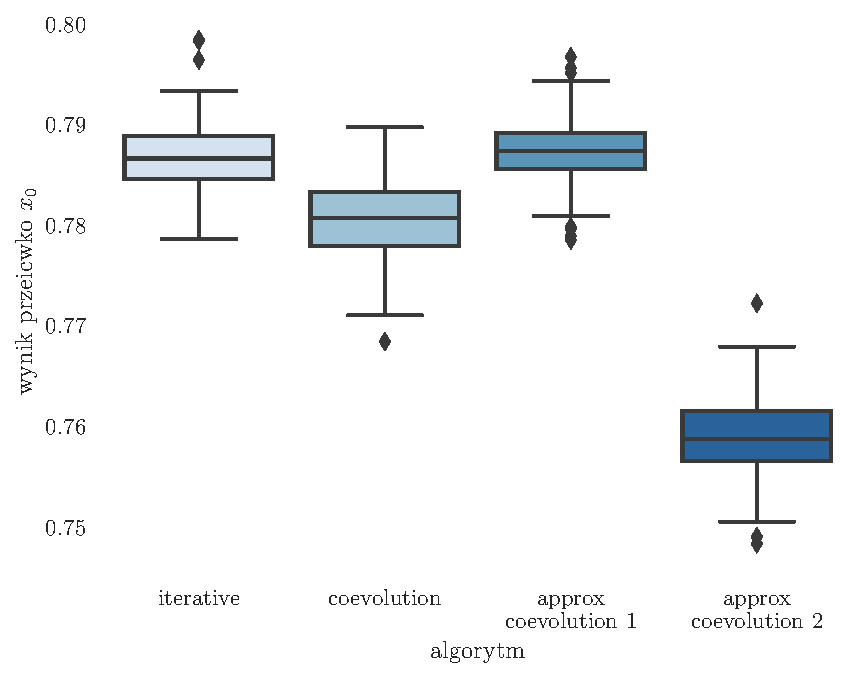
\includegraphics[width=0.79\textwidth]{imagens/war_results.pdf}
		%latinmodern w pythonie
		\caption{Wykresy pudełkowe przestawiające rezultaty uzyskanych strategii przeciwko strategii początkowej dla gry Wojna.}
		\label{fig:war_results}
	\end{figure}
\begin{table}
	\begin{center}
		\caption{Rezultaty uzyskanych strategii przeciwko losowej strategii początkowej dla gry Rrrats.}
		\small
		\begin{tabular}{lrrrr}
			\hline
			\toprule
			{} &  iterative &  coevolution &  approx coevolution 1 &  approx coevolution 2 \\
			\midrule
			mean  &    0,786629 &     0,780805 &             0,787310 &               0,759073 \\
			std   &    0,003581 &     0,004265 &             0,003586 &               0,004170 \\
			min   &    0,778600 &     0,768400 &             0,778500 &               0,748300 \\
			25\%   &    0,784550 &     0,777925 &             0,785575 &               0,756525 \\
			50\%   &    0,786600 &     0,780700 &             0,787350 &               0,758700 \\
			75\%   &    0,788800 &     0,783300 &             0,789125 &               0,761500 \\
			max   &    0,798400 &     0,789700 &             0,796700 &               0,772200 \\
			\bottomrule
			\hline
		\end{tabular}
		\caption*{\textit{Źródło: opracowanie własne}}
		
		\label{table:rrrats_results}
		\end{center}
	\end{table}
	\begin{table}
		\begin{center}
		\caption{Rezultaty uzyskanych strategii przeciwko losowej strategii początkowej dla gry Rrrats. Wartość po  ,,$\pm$'' jest odchyleniem standardowym.}
		\small
		\begin{tabular}{lllll}
			\hline
			\toprule
			{} &        iterative &      coevolution &    approx coevol 1&  approx coevol 2 \\
			\midrule
			iterative       &  0,519 $\pm$ 0,005 &  0,525 $\pm$ 0,005 &  0,518 $\pm$ 0,006 &  0,564 $\pm$ 0,004 \\
			coevolution     &  0,508 $\pm$ 0,005 &  0,515 $\pm$ 0,005 &  0,509 $\pm$ 0,005 &  0,555 $\pm$ 0,005 \\
			approx coevol 1  &  0,519 $\pm$ 0,005 &  0,525 $\pm$ 0,005 &  0,519 $\pm$ 0,005 &  0,565 $\pm$ 0,006 \\
			approx coevol 2 &  0,456 $\pm$ 0,005 &  0,464 $\pm$ 0,005 &  0,457 $\pm$ 0,005 &  0,507 $\pm$ 0,005 \\
			\bottomrule
			\hline
		\end{tabular}
		\caption*{\textit{Źródło: opracowanie własne}}
		\label{table:rrrats_results_all}
	\end{center}
\end{table}

	\begin{figure}
		\centering
		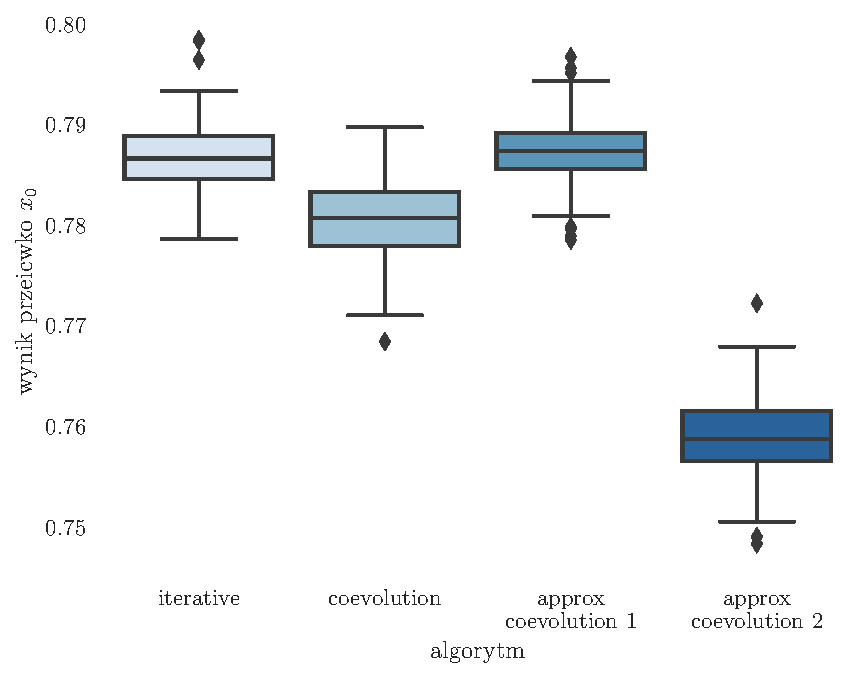
\includegraphics[width=0.79\textwidth]{imagens/rrrats_results.pdf}
		%latinmodern w pythonie
		\caption{Wykresy pudełkowe przestawiające rezultaty uzyskanych strategii przeciwko losowej strategii początkowej dla gry Rrrats.}
		\label{fig:rrrats_results}
	\end{figure}

	\newpage

	
	
{\backmatter \chapter{Podsumowanie}}
W pracy skupiliśmy się na analizie algorytmów typu Limited Empirical Bernstein Race, których głównym zadaniem jest szacowanie prawdopodobieństwa wygranej graczy.  W celu ulepszenia ich działania zaproponowaliśmy nowe algorytmy nazwane Improved Limited Empirical Bernstein Race. Poprzez analizę nierówności Hoeffdinga i empirycznej nierówności Bernsteina, określiliśmy maksymalną liczbę testów potrzebnych do zakończenia działania algorytmów typu ILEBR oraz wyznaczyliśmy wzór na prawdopodobieństwo popełnienia błędu dla badanych algorytmów. Ponadto opracowaliśmy metodę doboru parametrów początkowych, która pozwala ograniczyć ostateczny błąd do poziomu nieprzekraczającego żądanego prawdopodobieństwa $\alpha$. Wszystkie nasze teoretyczne rozważania zostały potwierdzone przez symulacje komputerowe.

Dodatkowo zastosowaliśmy te metody do algorytmów genetycznych oraz zaproponowaliśmy nowy algorytm generacyjny. Przy ich pomocy udało nam się symulacyjnie wyznaczyć optymalną strategię w testowanych dwuosobowych grach częściowo obserwowalnych. 


%{\backmatter \chapter{Dodatek}} \label{Dodatek}
{\appendix  \chapter[Dodatek]{}} 
\section{Dowód lematu \ref{lemma Bernstein race without maximum race length}}\label{proof:lemma Bernstein race without maximum race length}
\begin{proof}
	Niech $X_1, X_2, \dots, X_t$ będzie ciągiem i.i.d. zmiennych losowych, takim że $1$ i $0$ są odpowiednio górną i dolną granicą wartość zmiennej losowej $X_i$. Dodatkowo niech liczba rozegranych gier będzie funkcją zależną od $k$ ($f(k) = t$) %! czy pozbyc sie tego wtracenia
	oraz niech $\delta_k = \frac{\delta}{g(k)}$
	gdzie $\delta \ge \sum_{k=1}^{\infty} \frac{\delta}{g(k)}$ i $\ln(g(k)) \in o(f(k))$, wtedy z twierdzenia \ref{Popoviciu_ineq}
	\begin{gather}
		\label{proof:lemma Bernstein race without maximum race length 1}
		 \overline{\sigma}_t^2 \le \frac{1}{4}.
	\end{gather}
	Wykorzystując wynik \eqref{proof:lemma Bernstein race without maximum race length 1} do nierówności \eqref{Bernstein race without maximum race length} otrzymujemy 
	\begin{gather*}
		\epsilon_{f(k), k} \le  \sqrt{\frac{\ln(\frac{3g(k)}{\delta})}{2f(k)}} + \frac{3  \ln{(\frac{3g(k)}{\delta})}}{f(k)}.
	\end{gather*}
	Z założeń wiemy, że $\ln(g(k)) \in o(f(k))$, zatem
	\begin{gather*}
		\lim\limits_{k\to\infty} \frac{  \ln{(\frac{3g(k)}{\delta})}}{f(k)} = 0,
	\end{gather*}
	co ostatecznie z twierdzenia o trzech ciągach daje nam $ \lim\limits_{k\to\infty}  e_{f(k), k} = 0$.
\end{proof}

\section{Dowód nierówności (\ref{eq:error probability})}
\begin{proof}\label{proof:error probability}
	 Prawdopodobieństwo popełnienia błędu $\alpha$ jest równe sumie prawdopodobieństw pomyłki w momencie przeprowadzenia $k$-tego testu plus prawdopodobieństwo pomyłki po przeprowadzaniu $\nmax$ testów. Z założeń wiemy, że teoretyczna warowność $\mu > 0,5$. Zatem
	\begin{align*}
		\alpha=
		\probP&_{\mu}(\overline{X}_{f(1)} + \epsilon_{1} \le 0,5)  \\
		+&\probP_{\mu}(\overline{X}_{f(1)} + \epsilon_{1} > 0,5)\probP_{\mu}(\overline{X}_{f(2)} + \epsilon_{2} \le 0,5) \\
		+&\dots \\
		+&\probP_{\mu}(\overline{X}_{f(1)} + \epsilon_{1} > 0,5)\probP_{\mu}(\overline{X}_{f(2)} + \epsilon_{2} > 0,5)\cdots  \probP_{\mu}(\overline{X}_{f(\nmax)}+ \epsilon_{\nmax} \le 0,5)\\
		+&\probP_{\mu}(\overline{X}_{f(1)} + \epsilon_{1} > 0,5)\cdots  \probP_{\mu}(\overline{X}_{f(\nmax)}+ \epsilon_{\nmax} > 0,5)\probP_{\mu}(\overline{X}_{f(\nmax)} \le 0,5).
	\end{align*}
	Korzystając z prawdopodobieństwa zdarzenia przeciwnego otrzymujemy
	\begin{align*}
		\alpha=
		1& - \probP_{\mu}(\overline{X}_{f(1)} + \epsilon_{1} > 0,5) \\
		+&\probP_{\mu}(\overline{X}_{f(1)} + \epsilon_{1} > 0,5)(1 - \probP_{\mu}(\overline{X}_{f(2)} + \epsilon_{2} > 0,5)) \\
		+&\dots \\
		+&\probP_{\mu}(\overline{X}_{f(1)} + \epsilon_{1} > 0,5)\probP_{\mu}(\overline{X}_{f(2)} + \epsilon_{2} > 0,5)\cdots  (1-\probP_{\mu}(\overline{X}_{f(\nmax)}+ \epsilon_{\nmax} > 0,5))\\
		+&\probP_{\mu}(\overline{X}_{f(1)} + \epsilon_{1} > 0,5)\cdots  \probP_{\mu}(\overline{X}_{f(\nmax)}+ \epsilon_{\nmax} > 0,5)\probP_{\mu}(\overline{X}_{f(\nmax)} \le 0,5).
	\end{align*}
	Uzyskana suma upraszcza się przez teleskopowanie do postaci
	\begin{align*}
		\alpha =&  1- \prod^{\nmax}_{k=1} \probP_{\mu}(\overline{X}_{f(k)} +  \epsilon_{k} > 0,5)+ 
		\probP_{\mu}(\overline{X}_{f(\nmax)} \le 0,5)\prod^{\nmax}_{k=1} \probP_{\mu}(\overline{X}_{f(k)} +  \epsilon_{k} > 0,5)\\
		=& 1 - (1 - \probP_{\mu}(\overline{X}_{f(\nmax)} \le 0,5))
		\prod^{\nmax}_{k=1} \probP_{\mu}(\overline{X}_{f(k)} +  \epsilon_{k} > 0,5) \\
		=&1 -  \probP_{\mu}(\overline{X}_{f(\nmax)} > 0,5)
		\prod^{\nmax}_{k=1} \probP_{\mu}(\overline{X}_{f(k)} +  \epsilon_{k} > 0,5).
	\end{align*}
\end{proof}
\section{Dowód wyrażenia (\ref{eq:alpfa_determinant})}
\begin{proof}\label{proof:alpfa_determinant}
	Chcemy znaleźć minimalne $\nmax$, dla którego nasz błąd będzie nie większy niż żądane $\alpha$. Takie $\nmax$ będzie spełniać zależność 
	\begin{align}
		\label{eq:alpfa_determinant_n_max}
		\nmax =& \min \left\{n\in \mathbb{N}^+: F_{\mu}(n) < \alpha \right\}.
	\end{align}
	Podstawiając \eqref{eq:alpfa_determinant_n_max} do \ref{Hoeffding ineq lemma} otrzymujemy, że dla $\delta_k = \frac{\delta}{\nmax}$ i $t = f(\nmax)$
	\begin{align*}
		\epsilon \le  \sqrt{\frac{\ln(2\frac{\nmax}{\delta})}{2f(\nmax)}} \implies \delta \le   \cfrac{2\nmax}{\exp(2\epsilon^2f(\nmax))}.
	\end{align*}
\end{proof}


\bibliographystyle{bibliografia_styl}
\bibliography{bibliografia}
\end{document}